\documentclass[a4paper]{cas-sc}
\usepackage{multirow}
\usepackage{graphicx}
\usepackage[numbers,sort&compress]{natbib}
\let\printorcid\relax
\usepackage{float}
\usepackage{booktabs}
\usepackage{tabularx}
\usepackage{amsmath}
\usepackage{amsfonts}
\usepackage{url}
\usepackage{algorithm}
\usepackage{algpseudocode}
\newcommand{\PMS}{PMS}
\begin{document}
\let\WriteBookmarks\relax
\def\floatpagepagefraction{1}
\def\textpagefraction{.001}

\shorttitle{Causal-augmented Hierarchical LLMs for Building Control}

\shortauthors{W. Xin et~al.}

\newcommand{\revise}[1]{\textcolor{blue}{#1}}

\title [mode = title]{Causal-augmented Hierarchical LLM Agents for Building Control}

\author[1]{Weilin Xin}

\author[1]{Wei Liang}

\author[1]{Adrian Chong}
\cormark[1]
\cortext[cor1]{Corresponding author}

\affiliation[1]{organization={Department of the Built Environment, College of Design and Engineering, National University of Singapore},
    city={Singapore},
    postcode={117566},
    country={Singapore}}

\begin{abstract}
Multi-zone building HVAC control requires scalable methods that generalize across heterogeneous configurations without per-building retraining. Despite the potential of language-model-based multi-agent (LM-MA) frameworks, three challenges persist: unverified competitiveness against mainstream methods such as deep reinforcement learning (DRL), unclear applicability across heterogeneous HVAC configurations and control dimensions, and the absence of structural constraints to suppress physically implausible outputs. This study proposes a causal-augmented hierarchical control framework for zero-shot generalization. Informed by causal rules derived from building documentation, the framework adopts an LM-MA architecture that decouples control into strategic planning, safety-constrained execution, and closed-loop reflection with working memory. Experiments on three benchmark cases with distinct HVAC configurations yield 7.67--42.14\% cost savings over rule-based control. Compared with DRL, the framework performs competitively; in the best-performing dual-zone hydronic case, it achieves 6.26--13.54\% energy savings and reduces discomfort from 2.00--7.50 to 0.25 zone-hours. Ablation experiments show that single-hour working memory is most effective, and that causal augmentation reduces hallucination rates by up to 86.3\% while virtually eliminating safety violations. These results delineate the applicability boundaries of the hierarchical LM-MA framework, revealing more pronounced advantages when system thermal inertia exceeds the available prediction horizon. Collectively, these findings underscore the potential of causal augmentation for reliable language-model-based building control.
\end{abstract}

\begin{highlights}
\item Causal-augmented hierarchical framework enables zero-shot building HVAC control.
\item Performs competitively with deep reinforcement learning across three benchmarks.
\item Causal augmentation cuts hallucinations by 86.3\% and minimizes safety violations.
\item LLM agents show greater advantages in high thermal inertia systems.
\item Single-hour working memory is most effective across building configurations.
\end{highlights}

\begin{keywords}
Hierarchical multi-agent system \sep
Building HVAC control \sep
Causal augmentation \sep
Zero-shot generalization \sep
Large language model
\end{keywords}

\maketitle

% === SECTION 1: Introduction === %
\section{Introduction}

The building sector accounts for a substantial share of global end-use energy consumption, with heating, ventilation, and air conditioning (HVAC) systems representing the largest component of operational energy use~\cite{IEA2025-ger,Chua2013-xc}. Minimizing energy consumption while maintaining zone-level thermal comfort has therefore become a central research objective. However, multi-zone coordinated control is complicated by inter-zone thermal coupling arising from temperature differences and stochastic disturbances such as occupancy variations and time-varying electricity prices~\cite{Yang2020-yu,Liu2024-fd}. As the number of zones increases, the joint state--action space grows exponentially, further compounding optimal control~\cite{Lei2022-ni}. These challenges underscore the need for scalable, globally coordinated control strategies.

Two mainstream approaches address these challenges: optimization-based controllers such as model predictive control (MPC) and learning-based methods such as multi-agent reinforcement learning (MARL). Hierarchical and distributed MPC achieve scalability by decomposing the global problem into tractable subproblems~\cite{Rawlings2018-kk,Morosan2010-nd}, yet their deployment remains constrained by the cost of physical modeling and the computational overhead of online optimization~\cite{Drgo2020-faiel}. In contrast, MARL reduces reliance on explicit physical models and, under the centralized-training-with-decentralized-execution (CTDE) paradigm, enables zone-level agents to execute local control policies using local observations~\cite{Jendoubi2023-ak}. However, deep reinforcement learning (DRL) policies are typically coupled to the training environment and require retraining when transferred to new buildings. Achieving cross-building generalization in multi-zone control remains a key bottleneck.

Pre-trained large language models (LLMs) encode general world knowledge that enables adaptation to new buildings without retraining, offering a promising pathway for cross-building control~\cite{Shinn2023-ae}. Recent studies have demonstrated the feasibility of zero-shot building control using LLMs~\cite{Liu2025-ql}, and language-model-based multi-agent (LM-MA) frameworks have shown potential for scalable controller development~\cite{Hu2025-jb}. Nevertheless, three limitations persist in applying LM-MA frameworks to building control: (1) their competitiveness relative to data-driven baselines lacks systematic empirical evaluation; (2) the applicability conditions and performance boundaries across diverse HVAC configurations and control dimensions remain unclear; and (3) existing approaches lack domain-specific correction mechanisms for building physics constraints, exposing decisions to the risk of physically implausible outputs~\cite{Geissler2025-je} and undermining control reliability.

To address these gaps, this study proposes a causal-augmented hierarchical control framework comprising two operational phases and an independent audit module. In the offline causal initialization phase, the framework constructs a thermodynamic causal graph from building technical documentation and distills it into natural-language control rules, which serve as physical inductive biases embedded in the reasoning context. During online control, the hierarchical multi-agent architecture coordinates three specialized agents: the Orchestrator derives strategic directives from the global state and causal rules; the Executor translates these directives into control actions while enforcing deterministic safety constraints; and the Reflector evaluates execution outcomes and updates a sliding-window working memory with recent control history, thereby closing the control loop. An independent audit agent concurrently quantifies framework reliability through three behavioral metrics. By relying solely on offline causal initialization without building-specific training data, the framework achieves zero-shot generalization. To systematically evaluate its applicability conditions and performance boundaries, we compare the framework against both centralized and hierarchical DRL baselines across three heterogeneous building cases, and conduct ablation experiments to quantify the effects of causal augmentation and working memory window length on control performance and decision reliability.

The main contributions of this paper are as follows:
\begin{itemize}
    \item We propose a causal-augmented hierarchical control framework that integrates LLM reasoning with deterministic execution.
    \item We evaluate the framework across three heterogeneous building cases, demonstrating competitive performance relative to deep reinforcement learning baselines.
    \item We investigate the applicability conditions and zero-shot performance boundaries of the proposed framework across diverse HVAC configurations and control dimensions.
    \item We quantify the effects of core framework mechanisms, demonstrating that causal augmentation mitigates hallucinations while appropriate working memory ensures control stability.
\end{itemize}

The remainder of this paper is organized as follows. Section~\ref{sec:related_work} reviews related work. Section~\ref{sec:method} presents the proposed framework. Section~\ref{sec:experiments} describes the experimental setup. Section~\ref{sec:results} reports the results. Section~\ref{sec:discussion} discusses limitations and implications. Section~\ref{sec:conclusion} concludes the paper.

% === SECTION 2: Related Work === %
\section{Related Work}
\label{sec:related_work}

The central objective of multi-zone building HVAC control is to minimize global operational energy consumption while satisfying thermal comfort constraints in each zone. As the number of zones increases, the number of optimization variables grows approximately linearly, making centralized architectures increasingly susceptible to the computational burden of high-dimensional, non-convex optimization~\cite{Wu2015-os,Asad2017-je,Lu2005-vy}. Conventional distributed control systems (DCS) achieve rudimentary decentralization by delegating control tasks to zone-level controllers~\cite{Coffin1999-ddc}. However, their control logic is typically local, static, and reactive, with limited ability to anticipate future disturbances or coordinate cross-zone optimization at a higher level~\cite{Wang2020-bb,Manjavacas2024-no}. This limitation has driven the development of advanced control strategies with predictive and proactive coordination capabilities.

\subsection{Model predictive control}

Model predictive control (MPC) explicitly handles constraints and predicted disturbances through a receding-horizon approach, making it a mainstream framework for multi-zone building control. Existing methods primarily fall into two categories: hierarchical MPC and distributed MPC.

To improve scalability, hierarchical MPC decomposes the global optimization problem into manageable subproblems organized by decision level~\cite{Rawlings2018-kk,Riccardo2009-sc}. The architecture typically consists of an upper-level coordinator and lower-level local controllers: the coordinator optimizes building-level energy dispatch, while the local controllers determine zone-level heating or cooling actions under local constraints~\cite{Engel2024-pm,Khatibi2023-vg}. However, the upper-level controller cannot access zone-level constraints in real time, so its decisions may insufficiently capture local dynamics, thereby limiting control performance~\cite{Engel2024-pm}. Although explicitly integrating lower-level feedback into upper-level decisions can mitigate this issue~\cite{Engel2022-js}, it incurs additional communication and computational overhead.

In contrast to the vertical decomposition of hierarchical MPC, distributed MPC partitions the centralized optimization problem into multiple local subproblems, assigning each zone subsystem an independent local controller interconnected through communication links~\cite{Morosan2010-nd}. Algorithms such as the alternating direction method of multipliers (ADMM) or dual decomposition drive iterative negotiation among subsystems to approximate the global optimum without centralized computation~\cite{Su2020-qn,Li2021-ji}. However, this iterative process introduces significant communication overhead, and convergence speed degrades as the number of subsystems increases.

Despite their different decomposition strategies, both MPC paradigms share a structural bottleneck: reliance on explicit physical models. Physics-based modeling requires accurate system parameters and substantial domain expertise, leading to high deployment costs; moreover, even after problem decomposition, the computational burden of online optimization at each zone controller remains considerable. This bottleneck has motivated the rise of data-driven control methods that eliminate the need for explicit physical models.

\subsection{Deep reinforcement learning}

Deep reinforcement learning (DRL) bypasses explicit physical modeling by learning through direct agent--environment interaction. Algorithms such as PPO have been extensively validated for single-zone HVAC optimization~\cite{Liu2024-fk,Jiang2021-rg,Fu2023-zh}. To address dimensional growth in multi-zone settings, multi-agent reinforcement learning (MARL) assigns each decision unit an independent agent that acts on local observations. Early work predominantly adopted the independent learning paradigm, applying DQN and DDPG to discrete and continuous action-space energy management tasks, respectively~\cite{Prasad2019-vo,Lu2019-uf,Du2021-gj}. Under independent learning, however, each agent treats other agents as part of the environment, rendering the environment non-stationary from any single agent's perspective and severely limiting cross-agent coordination~\cite{Nguyen2020-ai,Canese2021-cw}.

To balance coordination with scalability, the centralized-training-decentralized-execution (CTDE) architecture was introduced. During training, a centralized critic estimates the global value function; during execution, decentralized actors rely solely on local observations for decision-making~\cite{Lee2020-dx,Jendoubi2023-ak}. Although CTDE alleviates the coordination problem, DRL methods in practice still face three limitations. First, DRL policies use the current observation as the sole decision input, limiting decision reliability under partial observability (POMDP)~\cite{Jendoubi2023-ak}. Second, continuous action outputs lack physical constraints, which in HVAC systems can cause frequent actuator switching and accelerated equipment wear~\cite{Wang2024-sk}. Third and most fundamentally, policies are fitted to specific building dynamics through extensive environment interaction, yielding poor generalization to out-of-distribution events~\cite{Fang2023-iz}.

The architectural selection dilemma further exacerbates this generalization limitation in multi-zone scenarios. When the number of zones is limited, centralized DRL (C-DRL) can model multi-zone joint control as a single optimization objective with global coordination capability~\cite{Savino2025-tt}; \citet{Zhou2025-ob} and \citet{Dai2026-qs} showed that hierarchical DRL (H-DRL) outperforms centralized approaches in high-dimensional settings through hierarchical decision decomposition. The systematic comparison by \citet{Pinto2022-bn} further corroborated this finding, demonstrating that the relative advantages of centralized and distributed architectures vary with climate conditions and building heterogeneity, and that no single architecture maintains optimal performance across all scenarios. The dependence of architectural choice on problem dimensionality, combined with the coupling of policies to specific environments, jointly motivates the search for alternative paradigms with cross-scenario generalization capability.

\subsection{Large language models in building control}

Large language models leverage general world knowledge and semantic reasoning acquired through pre-training to adapt to new scenarios without task-specific training, offering a potential pathway for cross-building generalization. Unlike MARL, which requires extensive online interaction with the target environment, LM-MA frameworks use natural language to facilitate inter-agent communication and collaboration, potentially decoupling control policies from specific building dynamics~\cite{Liu2025-ql,Sun2024-ig}.

Existing studies that introduce LM-MA into building control follow two main paths: assisted optimization and closed-loop control. On the assisted-optimization path, \citet{Li2025-gd} embedded an LLM within a rule-based control framework for photovoltaic-driven air conditioning, iteratively updating operational parameters through periodic feedback; \citet{Hu2025-jb} used building semantic models as input and employed two LLM agents to automatically generate PI controller code, demonstrating the potential of LLM-assisted controller development. However, in these assisted-optimization studies, the LLM operates at the controller design or periodic-update level rather than making step-level control decisions, and thus cannot adapt to building dynamics at operational time scales.

On the closed-loop control path, researchers have placed LLMs directly within real-time control loops. \citet{Ghorbanpour2025-icml} achieved performance exceeding that of RL in a data-center liquid-cooling task using a fine-tuned LLM, though this approach relies on scenario-specific fine-tuning data. \citet{Sawada2024-id} proposed an ``Office-in-the-Loop'' framework that realized multimodal-information-driven setpoint control in a real office, but generalization beyond that single scenario has not been verified. Furthermore, none of the above closed-loop studies address coordination among multi-zone agents. \citet{Liu2025-ql} initially explored this direction by constructing a three-tier agent architecture that decouples local intent generation from global energy coordination, demonstrating the logical feasibility of zero-shot multi-zone energy scheduling. However, that study was validated only under a single static operating condition, and its effectiveness in long-horizon dynamic scenarios remains unexamined.

In summary, existing LM-MA control frameworks have been validated primarily in single scenarios or static case studies, leaving two significant gaps: first, their competitiveness relative to data-driven baselines under long-horizon closed-loop conditions lacks verification; second, their applicability conditions and performance boundaries across heterogeneous HVAC configurations and varying state--action space scales remain unclear. To address these gaps, this study proposes a hierarchical LM-MA control architecture and conducts quantitative comparisons against data-driven baselines across three building cases with heterogeneous HVAC configurations.

\subsection{Physical reasoning reliability of LLMs}

The limited reliability of LLMs in physical reasoning constitutes a core barrier to their deployment in safety-critical control systems. The benchmark study by \citet{Geissler2025-je} showed that multiple leading models fail to achieve a 95\% accuracy threshold on undergraduate-level thermodynamics questions, revealing systematic deficiencies in the physical consistency of LLM outputs.

Two lines of research address this problem. The first employs multi-round feedback mechanisms to correct reasoning errors. \citet{Park2026-hc} proposed a multi-agent self-correction framework that iteratively improves physical reasoning through cross-validation among agents. The second augments the reasoning context with structured physical information retrieved from external knowledge bases via retrieval-augmented generation (RAG)~\cite{Liu2026-au}. However, the former relies on repeated inter-agent interaction, introducing communication overhead and decision latency problematic for real-time control; the latter depends on retrieval relevance, and inaccurate retrieval can degrade decision quality by introducing misleading information~\cite{Chen2023-bs}. More fundamentally, neither approach imposes structural constraints on LLM reasoning, making it difficult to systematically suppress physically implausible outputs. This gap provides the direct motivation for the causal augmentation mechanism proposed in this work.

% === SECTION 3: Method === %
\section{Method}
\label{sec:method}

This section details the proposed causal-augmented hierarchical multi-agent (LM-MA) control framework. As illustrated in Fig.~\ref{fig:overview}, unlike multi-agent reinforcement learning paradigms that rely on offline gradient updates and centralized value estimation (Fig.~\ref{fig:overview}a), the proposed framework adopts a semantic coordination paradigm (Fig.~\ref{fig:overview}b). An Orchestrator agent observes the global state and dispatches strategic directives; zone-level Executor agents translate these directives into control actions; and a Reflector agent analyzes execution outcomes and feeds structured summaries back to the Orchestrator, thereby closing the control loop without gradient updates.

\begin{figure}[pos=t]
    \centering
    
\includegraphics[width=\textwidth]{figs2/Figure1_Overview_Framework.jpg}
    \caption{Comparison of (a) the multi-agent reinforcement learning paradigm and (b) the proposed causal-augmented hierarchical control framework.}
    \label{fig:overview}
\end{figure}

Each agent comprises three core components: a large language model (LLM), tools, and working memory, enabling sustained interaction with the physical environment. To address the decision uncertainty and hallucination risks inherent in LLM-based physical control, the framework introduces an explicit causal augmentation mechanism. This mechanism constrains the LLM's reasoning boundaries using natural-language control rules distilled from a thermodynamic causal graph. Meanwhile, a working memory mechanism retains recent control history in a sliding window, compensating for the LLM's lack of persistent cross-step memory. The following subsections introduce the problem definition (Section~\ref{sec:problem_definition}), the hierarchical control framework (Section~\ref{sec:hierarchical_framework}), the causal augmentation mechanism (Section~\ref{sec:causal_augmentation}), and the working memory design (Section~\ref{sec:working_memory}).

\subsection{Problem definition}
\label{sec:problem_definition}

Consider a building containing $N_z$ controlled thermal zones, where each zone $i$ has an independent cooling temperature setpoint $u_i(t)$ as the control variable. The control objective is to minimize operational energy cost over a control horizon $T$ while satisfying thermal comfort constraints. This problem is formalized as the following constrained multi-objective optimization:

\begin{equation}
\min_{u_1, \ldots, u_{N_z}} \sum_{t=1}^{T} \left[ w_e \lambda_e \frac{C_t}{N_z} + \frac{w_c \lambda_c}{N_z} \sum_{i=1}^{N_z}\mathbb{I}(O_{t,i} > 0) \phi(\text{PMV}_{t,i}) + \frac{w_s \lambda_s}{N_z} \sum_{i=1}^{N_z} |\Delta u_{t,i}| \right]
\label{eq:objective}
\end{equation}

\noindent where $C_t$ denotes the energy cost at time step $t$; the indicator function $\mathbb{I}(O_{t,i} > 0)$ ensures that comfort penalties are computed only when zone $i$ is occupied ($O_{t,i} > 0$); $\phi(\text{PMV}_{t,i}) = \max(0, |\text{PMV}_{t,i}| - 0.5)^2$ is a nonlinear thermal comfort penalty function; and $|\Delta u_{t,i}|$ is the control action change, which penalizes abrupt setpoint adjustments to reduce equipment wear. The weight vector $\mathbf{w} = [w_e, w_c, w_s]$ is held constant across building cases, while scaling factors $\lambda$ normalize the numerical magnitudes (specific values are provided in Section~\ref{sec:experiments}). The control variable is subject to:

\begin{equation}
u_i(t) \in [T_{\min}, T_{\max}] = [20\,^{\circ}\text{C},\; 30\,^{\circ}\text{C}], \quad \forall\, i,\, t
\label{eq:constraint}
\end{equation}

The system state space comprises global and zone-level states. Global states include outdoor temperature $T_{\text{out}}$, solar irradiance $G$, electricity price $P_e$, and the corresponding $H$-step forecasts. Zone states include zone temperature $T_{\text{zone},i}$, occupancy $O_i$, and predicted mean vote $\text{PMV}_i$. To solve this multi-zone control problem, we model the system as a multi-agent system $\mathcal{M} = \{A_1, A_2, \ldots, A_n\}$, where each agent is defined as a triple:

\begin{equation}
A_i = (\mathcal{L}_i,\; \mathcal{T}_i,\; \mathcal{M}_i)
\label{eq:agent}
\end{equation}

\noindent Here, $\mathcal{L}_i$ is the large language model providing reasoning capability; $\mathcal{T}_i = \{t_1, \ldots, t_k\}$ is the tool set for interacting with the physical environment; and $\mathcal{M}_i$ is the memory module maintaining state information across decision steps.

\subsection{Hierarchical control framework}
\label{sec:hierarchical_framework}

The proposed hierarchical control framework consists of an offline preparation phase and an online control phase, with an independent audit module evaluating framework reliability. The offline phase constructs causal control rules that are provided as contextual input to the Orchestrator, as detailed in Section~\ref{sec:causal_augmentation}. This subsection focuses on the online control phase and the audit module, covering agent definitions, the hierarchical control loop algorithm, and the audit metrics.

\subsubsection{Agent definitions}

\textbf{Orchestrator agent.}
The Orchestrator performs global strategic planning on an hourly cycle. Its inputs include the current global state (weather forecasts, electricity prices), zone-level states (temperature, occupancy forecasts, PMV), causal control rules, and recent reflection records retrieved from the sliding window. From these inputs, the Orchestrator generates a JSON-formatted strategic directive for each thermal zone, containing a strategy description, reasoning rationale, and causal rule references. The prompt design is provided in Appendix Fig.~\ref{fig:closeloop_prompt}.

\begin{itemize}
    \item \textbf{LLM:} DeepSeek-chat
    \item \textbf{Tools:} (1) Observation parser---formats sensor data, weather forecasts, and occupancy curves into structured input; (2) Forecaster---provides $H$-step outlooks for weather, electricity price, and occupancy
    \item \textbf{Memory:} A sliding-window buffer of the most recent $k$ Reflector records. Each record contains: time index, mean setpoint, mean PMV, reward, evaluation label, and reflection text
\end{itemize}

\textbf{Executor agent.}
The Executor translates the Orchestrator's natural-language strategic directives into an executable Python control function \texttt{run\_control(obs)}, which accepts the current local observation and returns a cooling setpoint. Multiple Executor instances run in parallel across zones. The prompt design is provided in Appendix Fig.~\ref{fig:closeloop_prompt}.

\begin{itemize}
    \item \textbf{LLM:} DeepSeek-chat
    \item \textbf{Tools:} (1) Code executor---a Python sandbox environment that runs the generated control function; (2) Safety validator---enforces four hard safety constraints (detailed in Section~3.2.2)
    \item \textbf{Memory:} The Orchestrator's strategic directive serves as contextual input, updated hourly
\end{itemize}

\textbf{Reflector agent.}
The Reflector evaluates execution performance at the end of each hourly cycle and generates a structured semantic reflection following a [Context]$\rightarrow$[Action]$\rightarrow$[Outcome]$\rightarrow$[Lesson] causal narrative structure. Each reflection is accompanied by an evaluation label (POSITIVE / NEUTRAL / NEGATIVE) computed via deterministic rules (a PMV-based IF-THEN logic function) to prevent label hallucination. The prompt design is provided in Appendix Fig.~\ref{fig:closeloop_prompt}.

\begin{itemize}
    \item \textbf{LLM:} DeepSeek-chat
    \item \textbf{Tools:} (1) Reward calculator---computes energy cost, PMV-based comfort penalty, and smoothness penalty; (2) PMV evaluator---calls the pythermalcomfort library~\cite{Tartarini2020-ox} to compute thermal comfort indices
    \item \textbf{Memory:} Zone-level states and the Executor's actions and outcomes over the preceding hour
\end{itemize}

\subsubsection{Online control loop}

The online control phase employs a dual time-scale structure: an hourly strategic planning cycle and a 15-minute execution step. This design reflects building thermal inertia---temperature responses to setpoint changes typically require tens of minutes to hours~\cite{Braun1990-re}. High-level strategic reasoning is therefore constrained to the hourly scale, while the 15-minute execution step provides sufficient responsiveness for rapid transitions such as occupancy changes. Fig.~\ref{fig:infoflow} illustrates the information flow within a complete hourly cycle, and Algorithm~\ref{alg:control_loop} provides a formal description of the control loop.

\begin{figure}[pos=t]
    \centering
    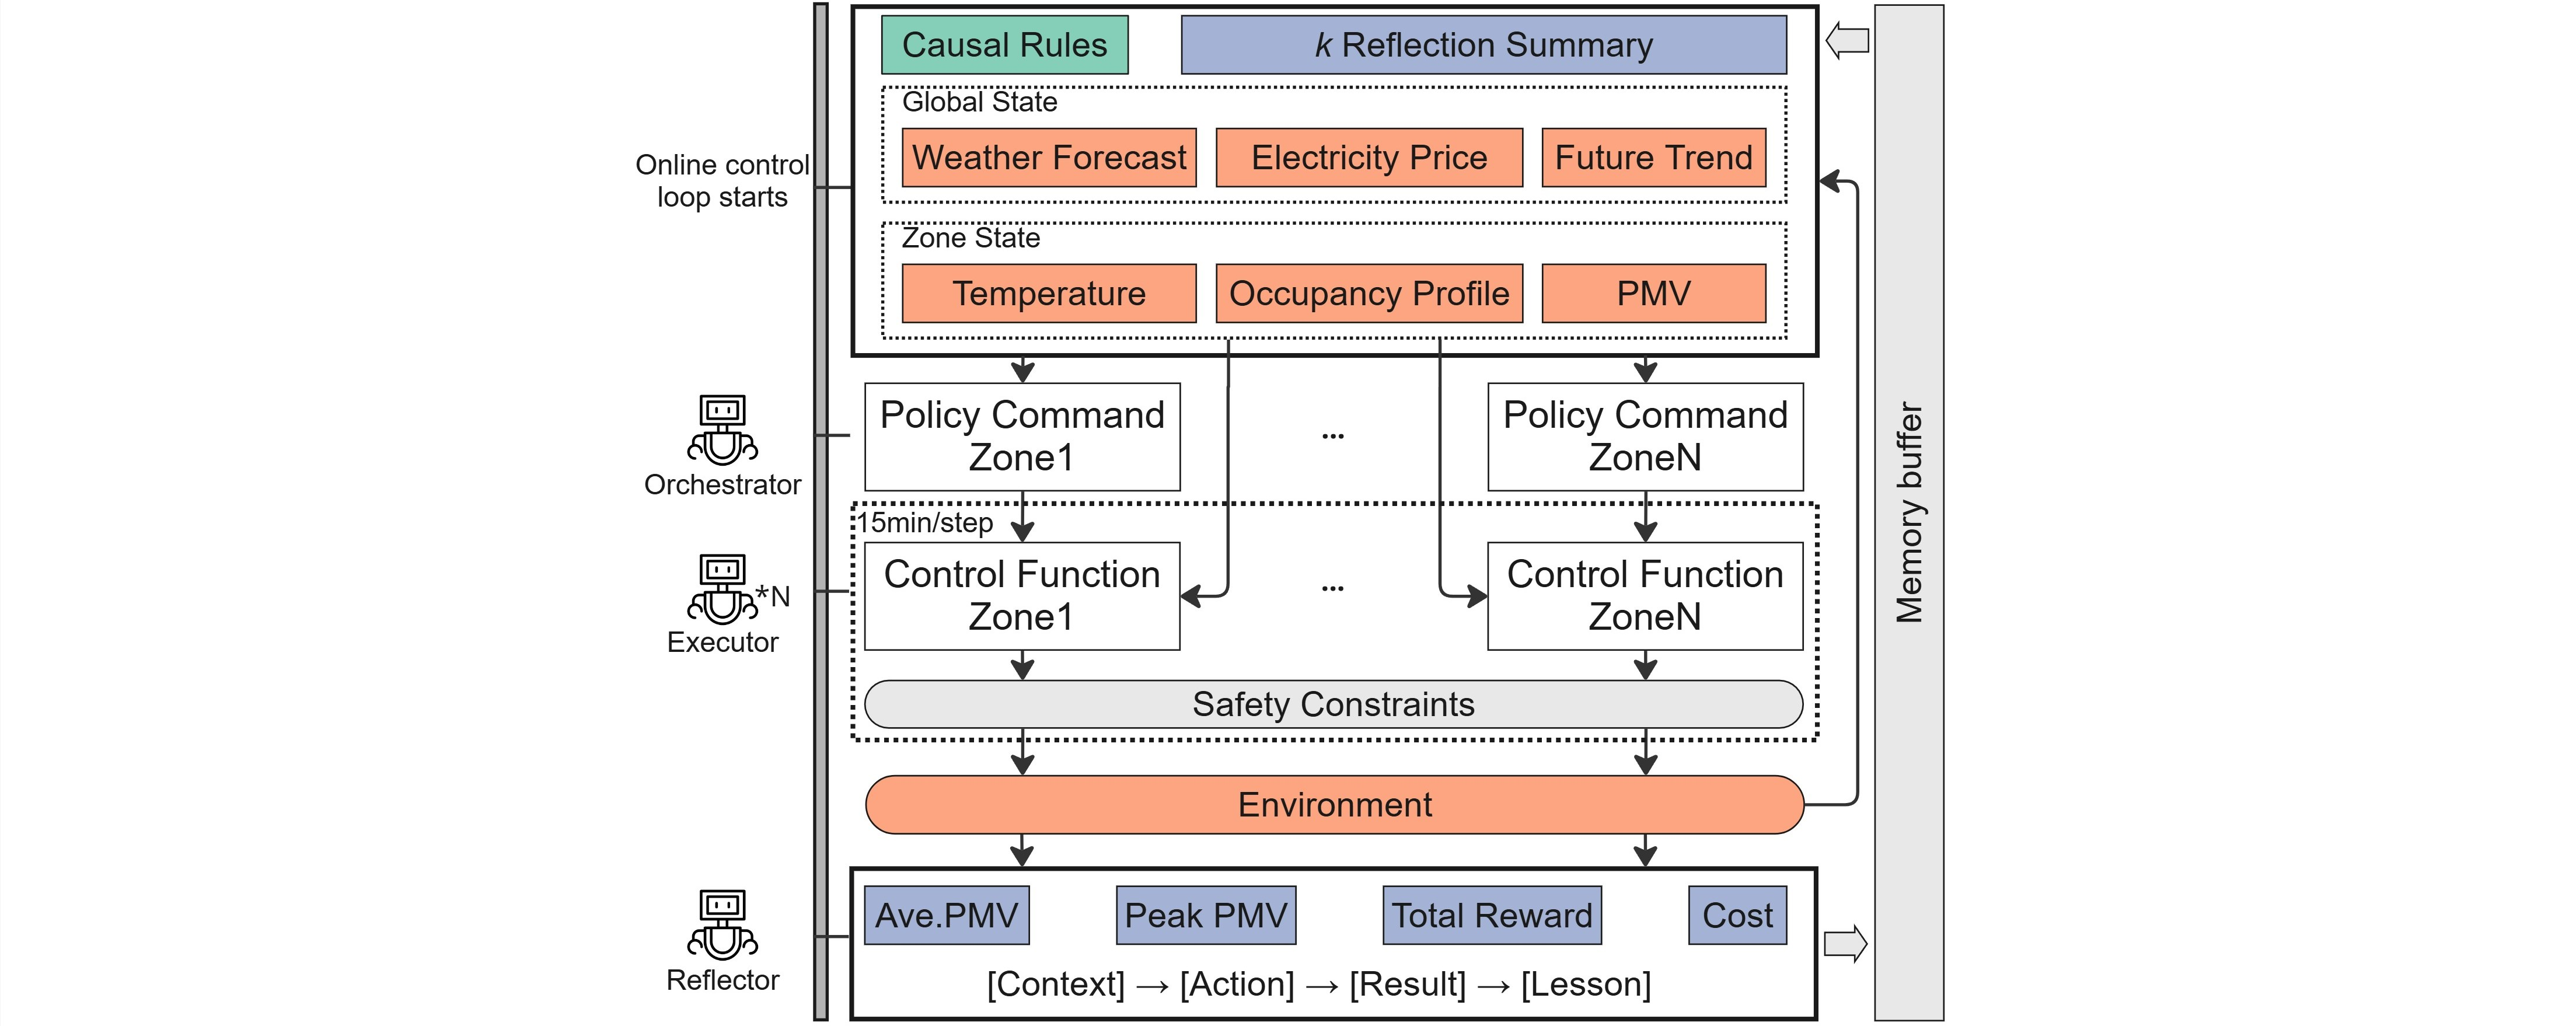
\includegraphics[width=\textwidth]{figs2/Figure2_Hourly_InfoFlow.jpg}
    \caption{Information flow within a single hourly control cycle, showing the observation and planning phase, execution and constraint phase, and reflection phase.}
    \label{fig:infoflow}
\end{figure}

\begin{algorithm}[t]
\caption{Hierarchical Control Loop}
\label{alg:control_loop}
\begin{algorithmic}[1]
\Require Building environment $\mathcal{E}$, causal rules $R$, window size $k$
\Ensure Setpoint sequence $\{u_i(s)\}$ for all zones

\State Run Causal Initialization (Sec.~3.3) \Comment{Offline}

\For{each hour $h = 1, \ldots, H$}
  \State $S_h \gets$ \textsc{Observe}(global state, zone states)
  \State $M_h \gets \{I_{h-k}, \ldots, I_{h-1}\}$ \Comment{Sliding window}
  \State $\{d_1, \ldots, d_{N_z}\} \gets f_O(S_h, F_h, R, M_h)$ \Comment{Orchestrator}

  \For{each step $s = 1, \ldots, 4$}
    \ForAll{zone $i$ \textbf{in parallel}}
      \State $u_i(s) \gets f_{E,i}(d_i, o_i(s))$ \Comment{Executor}
      \State $u_i(s) \gets \textsc{SafetyValidate}(u_i(s), o_i(s))$
    \EndFor
    \State Execute $\{u_i(s)\}$; measure $T_{\text{zone}}, P, \text{PMV}$
  \EndFor

  \State $I_h \gets \textsc{Reflect}(\text{hourly metrics})$ \Comment{Reflector}
  \State Append $I_h$ to sliding window
\EndFor
\end{algorithmic}
\end{algorithm}

At the beginning of each hourly cycle, the system enters the observation and planning phase. The Orchestrator aggregates global and zone-level states, while retrieving the most recent $k$ Reflector records from the sliding window as historical context. Synthesizing these inputs with the causal control rules $R$, the Orchestrator generates a strategic directive $d_i$ for each thermal zone. This process is formalized as the mapping $f_O: (S_h, F_h, R, M_h) \rightarrow \{d_1, \ldots, d_{N_z}\}$. Each directive is encoded in JSON format and contains a strategy description (e.g., comfort-constrained pre-occupancy pre-cooling), a reasoning rationale, and causal rule references, providing the execution layer with explicit and traceable control intent.

Strategic directives then enter the execution and constraint phase. Within each 15-minute step of the current hour, zone-level Executor agents run in parallel, translating the corresponding directive $d_i$ and current local observation $o_i(s)$ into an executable Python control function \texttt{run\_control(obs)} that outputs a cooling setpoint $u_i(s) = f_{E,i}(d_i, o_i(s))$. This code-generation-based execution approach---as opposed to direct numerical output---enables explicit conditional branching in the control logic, allowing dynamic responses to real-time occupancy states and PMV feedback within the 15-minute step.

However, LLM-generated code inherently carries the risk of logical errors. To mitigate this risk, the execution layer embeds four deterministic hard safety constraints that operate independently of LLM reasoning, forming a safety barrier between probabilistic inference and the physical system: (1)~\textit{Safety interlock}---when occupancy persists and PMV exceeds the comfort threshold ($|\text{PMV}| > 0.5$), the setpoint is forced to 25.0\,$^{\circ}$C to prevent sustained comfort violations; (2)~\textit{State anchoring}---during steady-state occupancy, single-step adjustment magnitude is limited to 0.5--1.0\,$^{\circ}$C relative to the previous setpoint, with the baseline reset to 25.0\,$^{\circ}$C upon occupancy transitions, preventing numerical oscillations in high-gain systems; (3)~\textit{Unoccupied baseline}---when both current and next-hour occupancy are zero, the setpoint defaults to 30.0\,$^{\circ}$C to ensure baseline energy efficiency; (4)~\textit{Pre-cooling logic}---when the zone is currently unoccupied but forecast to be occupied in the next hour, pre-cooling is initiated to exploit building thermal mass in preparation for upcoming occupancy, with intensity modulated by the thermal inertia label in the causal rules. After constraint validation, all setpoints are clipped to $[20,\,30]\,^{\circ}$C and dispatched to the building simulation environment.

At the end of each hourly cycle, the system enters the reflection phase. The Reflector aggregates execution data from the preceding hour---mean PMV, peak PMV, total reward, and energy cost---and generates a structured semantic reflection following the [Context]$\rightarrow$[Action]$\rightarrow$[Outcome]$\rightarrow$[Lesson] causal narrative structure. This reflection is then stored in the sliding-window buffer for the Orchestrator's use in the next hourly cycle, thereby closing the plan--execute--reflect control loop.

\subsubsection{Agent behavior evaluation}

The agent behavior audit module operates as an independent post-hoc observer, separate from the control loop, to quantitatively assess decision reliability. The audit agent parses the Orchestrator's reasoning logs alongside synchronized environmental state data to detect logical contradictions between reasoning and physical facts. The prompt design and output examples are provided in Appendix Fig.~\ref{fig:audit_prompt}. We define three complementary audit metrics:

\textbf{Hallucination Rate ($R_H$):}

\begin{equation}
R_H = \frac{1}{T} \sum_{t=1}^{T} \mathbb{I}(\text{Reasoning}_t \not\cong \text{State}_t)
\label{eq:hallucination}
\end{equation}

\noindent where $\mathbb{I}(\cdot)$ is the indicator function. This metric measures the proportion of time steps in which the Orchestrator's reasoning contradicts the actual physical state.

\textbf{Semantic Jitter ($J$):}

\begin{equation}
J = \frac{1}{T-1} \sum_{t=1}^{T-1} (1 - \text{CosSim}(\mathbf{v}_t, \mathbf{v}_{t-1}))
\label{eq:jitter}
\end{equation}

\noindent where $\mathbf{v}_t$ is the text embedding vector of the control policy at time step $t$. This metric quantifies temporal fluctuations of the control policy in the semantic space.

\textbf{Safety Intervention Rate ($R_{\text{SIR}}$):}

\begin{equation}
R_{\text{SIR}} = \frac{1}{T} \sum_{t=1}^{T} \mathbb{I}(|A_{\text{code},t} - S_{\text{trend},t}| > \delta)
\label{eq:sir}
\end{equation}

\noindent where $A_{\text{code}}$ is the Executor agent's actual output, $S_{\text{trend}}$ is the Orchestrator's intended direction, and $\delta$ is the deviation threshold. This metric measures how frequently the hierarchical safety mechanism overrides the high-level strategy. Together, the three metrics provide complementary perspectives on reasoning quality, policy stability, and safety layer effectiveness.

\subsection{Causal augmentation}
\label{sec:causal_augmentation}

LLM reasoning is fundamentally probabilistic: given an input context, the model generates the most likely output based on statistical regularities in its training corpora. When applied to building control, this probabilistic reasoning lacks an intrinsic understanding of thermodynamic causal relationships---the model may generate semantically plausible but physically infeasible strategies (e.g., implementing aggressive deep pre-cooling in a high-inertia hydronic system). The proposed framework addresses this by constructing an offline thermodynamic causal graph from building documentation and distilling it into natural-language control rules, which are statically embedded as physical inductive biases in the Orchestrator's reasoning context. These rules incur no additional runtime computational overhead and, because they are grounded in causal structure rather than statistical correlation, effectively constrain the LLM's reasoning to the physically feasible domain.

The causal augmentation module operates as an offline preprocessing pipeline that transforms building technical documentation into actionable physical priors. Its workflow, illustrated in Fig.~\ref{fig:causal_init}, comprises three steps: variable standardization (Section~3.3.1), causal graph construction (Section~3.3.2), and rule distillation (Section~3.3.3).

\begin{figure}[pos=t]
    \centering
    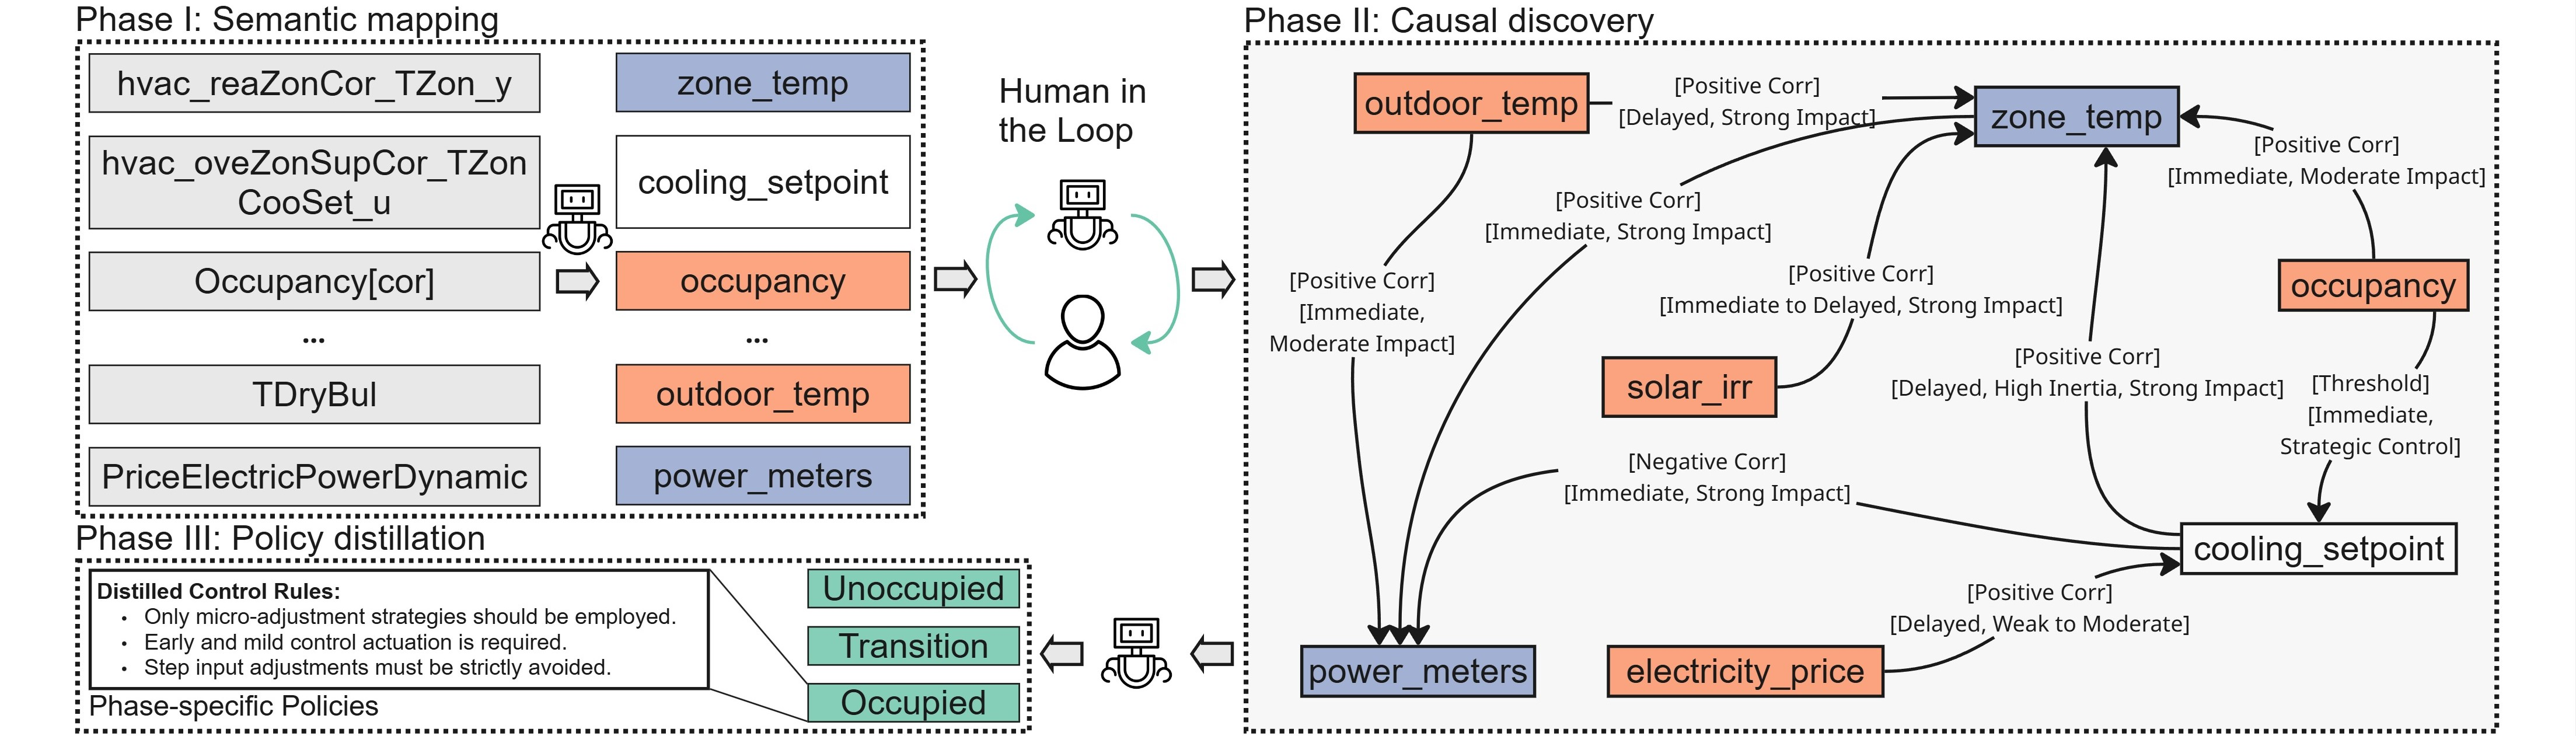
\includegraphics[width=\textwidth]{figs2/Figure3_Causal_Initialization.jpg}
    \caption{Causal initialization workflow: semantic mapping, causal graph construction via human-in-the-loop iteration, and rule distillation.}
    \label{fig:causal_init}
\end{figure}

\subsubsection{Semantic mapping}

Different buildings employ heterogeneous variable naming conventions in their building management systems (BMS) (e.g., \texttt{hvac\_reaZonCor\_TZ\_on\_y}), which hinders framework transfer across buildings. The Mapper agent uses an LLM to parse unstructured building technical documentation (BMS point lists, equipment specifications) into a standardized JSON data dictionary. We predefine a universal JSON Schema specifying key physical variables at both zone level---\texttt{cooling\_setpoint}, \texttt{zone\_temp}, \texttt{occupancy}---and global level---\texttt{outdoor\_temp}, \texttt{solar\_irr}, \texttt{electricity\_price}, \texttt{power\_meters}. The agent prompt and JSON Schema are provided in Appendix Fig.~\ref{fig:mapper_prompt}.

Given this predefined structure, the Mapper agent automatically classifies and semantically aligns raw BMS variables. For example, in the single-zone all-air case, the raw variable \texttt{fcu\_reaTZon\_y} is mapped to the standard name \texttt{zone\_temp}. This step eliminates ambiguity caused by inconsistent naming across heterogeneous buildings, providing a unified interface for downstream reasoning.

\subsubsection{Causal graph construction}

Building on the standardized variables, the Causal Discovery agent constructs a building thermodynamic causal graph (prompt design provided in Appendix Fig.~\ref{fig:causal_prompt}). This graph is directed and qualitative---unlike Bayesian networks or structural equation models, it encodes neither probability distributions nor precise quantitative relationships, but rather domain knowledge about causal direction and physical response characteristics between variables.

Each causal edge follows the format:

\begin{equation}
\texttt{cause variable} \xrightarrow{[\text{Relationship type}]} \texttt{effect variable} \quad [\text{Attribute labels}]
\label{eq:causal_edge}
\end{equation}

\noindent where the relationship type is one of Positive Correlation, Negative Correlation, or Threshold; dynamic attributes specify Immediate or Delayed response; and sensitivity attributes specify Strong Impact, Weak Impact, or High Inertia. For example, a causal edge in the dual-zone hydronic case is:

$$\texttt{cooling\_setpoint} \xrightarrow{[\text{Positive Corr}]} \texttt{zone\_temp} \quad [\text{Delayed, High Inertia}]$$

\noindent This encodes the physical knowledge that lowering the cooling setpoint reduces zone temperature, but the response exhibits significant delay and inertia due to the large thermal mass of the hydronic system.

Causal graph construction employs a human-in-the-loop iterative mechanism: (1)~the LLM proposes an initial causal graph based on the standardized variable list and building type; (2)~a domain expert reviews the physical plausibility of each causal chain; (3)~the expert provides specific critiques (e.g., ``the solar irradiance effect on the south zone should be labeled Strong Impact''); (4)~the LLM revises the graph accordingly; and (5)~steps 2--4 are repeated until the expert approves the final graph. This iterative process ensures that the generated causal chains conform to thermodynamic principles, correcting LLM reasoning inaccuracies under specific operating conditions.

\subsubsection{Rule distillation}

The approved causal graph is subsequently transformed into actionable strategic control rules. The key insight of this distillation process is that causal edge attributes must be reinterpreted through a control-theoretic lens rather than translated by common-sense intuition. Specifically, ``Strong Impact'' does not imply ``adjust aggressively'' but rather indicates high system gain---small setpoint changes produce large temperature responses, necessitating fine-grained adjustments to avoid overshoot. ``Delayed'' does not imply ``increase the magnitude'' but rather signals system lag---aggressive current adjustments will cause future overshoot, necessitating early but moderate action. ``High Inertia'' indicates that the system resists change, requiring avoidance of large step inputs. This interpretation framework constitutes the core control logic of rule distillation.

The Rule Distiller agent transforms the causal graph into strategic control rules using this framework (prompt and output examples provided in Appendix Fig.~\ref{fig:rule_prompt}). Because any occupied building exhibits three operational phases---unoccupied, occupancy transition, and steady-state occupancy---the distilled rules are organized by these three phases. The rule content for each phase is determined by the causal graph edge attributes and thus varies with building type. For instance, in the dual-zone hydronic case, the High Inertia and Delayed attributes produce rules that initiate pre-cooling early but with conservative magnitude to avoid overshoot. The Strong Impact (high-gain) attribute further constrains occupied-period adjustments to small increments, as the high-gain cooling response combined with solar irradiance disturbances can readily induce oscillations. In contrast, low-inertia all-air systems yield rules with shorter pre-cooling lead times and more responsive occupied-period adjustments.

This differentiation exemplifies the value of causal-graph-driven rule distillation. The same control-theoretic interpretation framework, acting on different causal structures, automatically generates strategic rules matched to building physical characteristics. The distilled rules are injected into the Orchestrator's context in natural language as physical priors, constraining its reasoning space to the feasible domain defined by thermodynamic causal relationships.

\subsection{Working memory}
\label{sec:working_memory}

Large language models are inherently stateless---they retain no information between invocations, and any memory across decision cycles must be explicitly provided as input at each step. However, the thermal response of building HVAC systems exhibits significant lag, requiring temporal context to identify temperature drift trends, detect setpoint oscillation patterns, and evaluate the effectiveness of prior strategies. To bridge the gap between the LLM's stateless nature and the temporal requirements of thermal systems, the framework employs a short-term sliding window as a working memory mechanism. At the end of each hourly cycle, the Reflector generates a structured performance reflection and appends it to a fixed-size buffer.

Each reflection record $I_h$ contains the time index $h$, mean cooling setpoints across zones, mean PMV of occupied zones, total reward for the hour, a deterministic evaluation label, and a reflection text following the [Context]$\rightarrow$[Action]$\rightarrow$[Outcome]$\rightarrow$[Lesson] causal narrative structure. The working memory is formally defined as:

\begin{equation}
M_h = \{I_{h-k}, \ldots, I_{h-1}\}
\label{eq:memory}
\end{equation}

\noindent where $k$ is the lookback window length. The framework uses only short-term sliding-window memory without long-term memory or retrieval-augmented generation (RAG). The primary operational time scales of building thermodynamics range from minutes to hours, so the most valuable information for control decisions is the recent operational trajectory---whether setpoints caused overshoot, whether comfort is trending toward violation, and whether the current strategy is effective. Longer-term patterns (seasonal trends, weekly regularities) are already captured through temporal encoding and static causal rules. The working memory window size $k$ is a key design parameter of this framework. In Section~5.3, we systematically analyze the effects of $k$ on control performance, computational cost, and decision stability, providing empirical guidance for sliding-window design.

% === SECTION 4: Experimental Setup === %
\section{Experimental Setup}
\label{sec:experiments}

\subsection{Simulation platform and case studies}

We adopt the Building Optimization Testing Framework (BOPTEST)~\cite{Blum2021-nx} as the simulation platform. BOPTEST constructs high-fidelity building thermodynamic models using the Modelica language and provides standardized RESTful APIs for control algorithm interaction, establishing a unified testing infrastructure for fair comparison. To evaluate the generalization and performance of the proposed framework across heterogeneous building environments, we select three representative benchmark cases covering single-zone and multi-zone layouts with both all-air and hydronic HVAC configurations. Table~\ref{tab:cases} summarizes the specifications and simulation periods for each case.

\begin{table}[htbp]
    \centering
    \caption{Overview of BOPTEST benchmark cases.}
    \label{tab:cases}
    \renewcommand{\arraystretch}{1.3}
    \begin{tabularx}{\textwidth}{l c l c c c}
        \toprule
        \textbf{Case} & \textbf{Zones} & \textbf{HVAC Type} & \textbf{Sim. Start (day)} & \textbf{Eval. Start (day)} & \textbf{Eval. Duration (days)} \\
        \midrule
        \texttt{SZ\_Air}   & 1 & Ideal VAV           & 196 & 203 & 7 \\
        \texttt{MZ\_Hydro} & 2 & FCU + Chiller/HP    & 213 & 220 & 5 \\
        \texttt{MZ\_Air}   & 5 & VAV + AHU           & 192 & 198 & 7 \\
        \bottomrule
    \end{tabularx}
\end{table}

The three cases emphasize distinct control challenges. \texttt{SZ\_Air} is a single-zone ideal all-air system near Denver, CO, USA (Appendix Fig.~\ref{fig:schematic_sz}) with low thermal inertia and rapid disturbance responses, serving to verify basic control capability in fast-response scenarios. \texttt{MZ\_Hydro} is a dual-zone hydronic system in Belgium (Appendix Fig.~\ref{fig:schematic_mz_hydro}) with high thermal inertia, inter-zone thermal coupling, and lagged solar irradiance response, placing greater demands on pre-cooling strategies and inertia-aware control. \texttt{MZ\_Air} is a five-zone all-air system in Chicago, IL, USA (Appendix Fig.~\ref{fig:schematic_mz_air}) with the highest dimensionality and cross-zone coupling, primarily testing scalability for high-dimensional multi-zone coordination.

Across all cases, the control variable is defined as the cooling temperature setpoint $T_{\text{set,c}}$ for each controlled zone, with the action space constrained to $[20\,^{\circ}\text{C},\,30\,^{\circ}\text{C}]$ (Eq.~(\ref{eq:constraint})). To focus on active cooling-season control strategies, the heating setpoint is fixed at 15\,$^{\circ}$C. For all-air cases (\texttt{SZ\_Air} and \texttt{MZ\_Air}), the supply air temperature is fixed at 17\,$^{\circ}$C and agents adjust only the terminal zone setpoints; for the hydronic case (\texttt{MZ\_Hydro}), agents directly adjust fan coil unit zone setpoints. All control actions execute at 15-minute intervals. The simulation environment incorporates a dynamic electricity pricing mechanism to incentivize exploitation of building thermal mass for pre-cooling during off-peak periods.

\subsection{Baselines and experimental implementation}

\subsubsection{Rule-based baseline (RBC)}

We adopt a standard occupancy-scheduled rule-based control (RBC) strategy as the reference baseline. This strategy follows a binary logic common in industry practice: during occupied periods, cooling setpoints for all zones are maintained at the comfort temperature of 25\,$^{\circ}$C; during unoccupied periods, setpoints are relaxed to the energy-saving temperature of 30\,$^{\circ}$C.

\subsubsection{Deep reinforcement learning baselines (DRL)}

We employ two classes of PPO-based deep reinforcement learning agents as data-driven baselines, representing two architectural choices for multi-zone control. The first is centralized DRL (C-DRL): a single-agent PPO that concatenates observations from all controlled zones into a global state, with a single policy network directly outputting joint actions for all zones. The second is hierarchical DRL (H-DRL): multi-agent PPO (MAPPO) using a CTDE architecture---a centralized critic receives the global state to estimate the value function, while decentralized actors output control actions independently based on local observations. For the single-zone case (\texttt{SZ\_Air}), only C-DRL is deployed as multi-agent coordination is unnecessary; for multi-zone cases (\texttt{MZ\_Hydro} and \texttt{MZ\_Air}), both C-DRL and H-DRL are deployed.

To accelerate training convergence and ensure policy safety during early exploration, DRL agents adopt a residual control architecture: their output is a setpoint offset $\Delta u_t$ relative to the RBC baseline rather than an absolute setpoint value. To capture system thermal inertia and enable anticipatory control, we design a high-dimensional observation space with symmetric temporal windows. Table~\ref{tab:obs} details the feature composition. The observation space combines the past $H$ steps of historical states with $H$-step environmental forecasts ($H = 4$, corresponding to a one-hour horizon). Network architecture and training hyperparameters are listed in Table~\ref{tab:hyperparams}. DRL models complete training in the simulation environment before the evaluation period (7 simulation days for \texttt{SZ\_Air} and \texttt{MZ\_Air}, 5 days for \texttt{MZ\_Hydro}), ensuring fully converged policies (convergence curves are provided in Appendix Fig.~\ref{fig:convergence}).

\begin{table}[htbp]
    \centering
    \caption{DRL observation space features.}
    \label{tab:obs}
    \renewcommand{\arraystretch}{1.3}
    \begin{tabularx}{\textwidth}{l X c l}
        \toprule
        \textbf{Feature} & \textbf{Description} & \textbf{Temporal Window} & \textbf{Physical Meaning} \\
        \midrule
        Time encoding    & $\sin(t),\;\cos(t)$           & Current           & Diurnal/weekly periodicity \\
        Zone state       & $T_{\text{zone}}$             & Current + past 4  & Thermal inertia and comfort \\
        Comfort          & PMV                            & Current           & Real-time thermal comfort \\
        System state     & $P_{\text{sys}}$ (normalized)  & Past 4            & Historical power trend \\
        Historical action & $\Delta u_{\text{cool}}$      & Past 4            & Action smoothness \\
        Weather forecast & $T_{\text{out}}$, GHI          & Current + next 4  & Outdoor temperature and solar outlook \\
        Disturbance forecast & Occupancy, electricity price & Current + next 4 & Occupancy schedule and dynamic pricing \\
        \bottomrule
    \end{tabularx}
    \begin{flushleft}
        \footnotesize
        \textbf{Note:} For MAPPO multi-zone cases, the table describes the global observation space used by the Critic. Each Actor's local observation is a subset containing time encoding, its own zone state/PMV/action history, shared system power, shared weather/price forecasts, and its own occupancy forecast.
    \end{flushleft}
\end{table}

\begin{table}[htbp]
    \centering
    \caption{DRL hyperparameter configuration.}
    \label{tab:hyperparams}
    \renewcommand{\arraystretch}{1.3}
    \setlength{\tabcolsep}{4pt}
    \footnotesize
    \begin{tabular}{l c c c c c}
        \toprule
        \textbf{Hyperparameter} & \makecell{\texttt{SZ\_Air}\\(PPO)} & \makecell{\texttt{MZ\_Hydro}\\(C-DRL)} & \makecell{\texttt{MZ\_Hydro}\\(H-DRL)} & \makecell{\texttt{MZ\_Air}\\(C-DRL)} & \makecell{\texttt{MZ\_Air}\\(H-DRL)} \\
        \midrule
        Actor LR          & $5.0\!\times\!10^{-4}$ & $3.0\!\times\!10^{-4}$ & $3.0\!\times\!10^{-4}$ & $3.0\!\times\!10^{-4}$ & $3.0\!\times\!10^{-4}$ \\
        Critic LR         & ---                     & ---                     & $5.0\!\times\!10^{-4}$ & ---                     & $5.0\!\times\!10^{-4}$ \\
        Entropy coeff.    & 0.02 & 0.02 & 0.01 & 0.02 & 0.01 \\
        Update epochs     & 10   & 10   & 10   & 10   & 10 \\
        Batch size        & 168  & 120  & 120  & 168  & 168 \\
        Network           & [256, 256] & [256, 256] & [256, 256] & [256, 256] & [256, 256] \\
        Steps / epochs    & 672 / 300  & 480 / 300  & 480 / 300  & 672 / 300  & 672 / 300 \\
        Discount $\gamma$ & 0.99 & 0.99 & 0.99 & 0.99 & 0.99 \\
        GAE $\lambda$     & 0.95 & 0.95 & 0.95 & 0.95 & 0.95 \\
        Gradient clip     & 0.5  & 0.5  & 0.5  & 0.5  & 0.5 \\
        \bottomrule
    \end{tabular}
\end{table}

\subsubsection{Fair comparison design}

To ensure fair comparison, performance evaluation for all strategies is conducted within the same evaluation period defined in Table~\ref{tab:cases}. The DRL baselines (C-DRL and H-DRL) require a training phase prior to evaluation, whereas the RBC baseline and the proposed framework are deployed directly in zero-shot mode. The proposed framework relies solely on offline causal rules (Section~3.3) and the runtime Reflector feedback mechanism for control decisions. All strategies share a unified reward function (Eq.~(\ref{eq:objective})) and dynamic electricity pricing mechanism. The reward function weights are $\mathbf{w} = [w_e, w_c, w_s] = [1.0, 20.0, 0.1]$ across all cases; scaling factors $\lambda$ are listed in Table~\ref{tab:scaling}.

\begin{table}[htbp]
    \centering
    \caption{Reward function scaling factors.}
    \label{tab:scaling}
    \renewcommand{\arraystretch}{1.3}
    \begin{tabular}{l c c c c}
        \toprule
        \textbf{Parameter} & \textbf{Symbol} & \texttt{SZ\_Air} & \texttt{MZ\_Hydro} & \texttt{MZ\_Air} \\
        \midrule
        Energy scaling   & $\lambda_e$ & 120.35 & 3.0  & 18.53 \\
        Comfort scaling  & $\lambda_c$ & 10.0   & 0.75 & 10.0 \\
        Smoothness scaling & $\lambda_s$ & 0.18 & 0.18 & 0.38 \\
        \bottomrule
    \end{tabular}
\end{table}

\subsection{Evaluation metrics}

Thermal comfort is assessed using Fanger's predicted mean vote (PMV) model, computed via the pythermalcomfort library~\cite{Tartarini2020-ox}. We specify standardized physical parameters: metabolic rate of 1.1~met, relative humidity of 50\%, and indoor air velocity of 0.1~m/s. Mean radiant temperature ($T_{\text{mrt}}$) is approximated as indoor air temperature for all-air system cases and as operative temperature for the hydronic case. For the two all-air cases (\texttt{SZ\_Air} and \texttt{MZ\_Air}), clothing insulation ($I_{\text{clo}}$) follows a dynamic model that linearly interpolates between 0.5~clo (summer) and 1.0~clo (winter) based on the daily mean outdoor temperature (thresholds of 26\,$^{\circ}$C and 10\,$^{\circ}$C), simulating occupant adaptation to seasonal changes. For \texttt{MZ\_Hydro}, dynamic clothing insulation would produce high-frequency PMV target fluctuations that impede policy convergence. To focus evaluation on control strategy performance in high-lag systems, all methods (RBC, both DRL baselines, and the proposed framework) use a fixed summer-typical value of $I_{\text{clo}} = 0.5$~clo for this case.

We compare experimental results through three core physical metrics. Total energy consumption measures the cumulative electricity consumption (kWh) of the HVAC system over the evaluation period. Total cost combines dynamic electricity prices to compute cumulative operational expenditure. Discomfort duration is defined as cumulative zone-hours: at each time step during occupied periods, the number of zones in a discomfort state ($|\text{PMV}| > 0.5$) is counted and accumulated, quantifying localized comfort violations in multi-zone environments. These physical metrics complement the agent behavior audit metrics defined in the Method section (Eqs.~(\ref{eq:hallucination})--(\ref{eq:sir})), providing a comprehensive evaluation across both physical control effectiveness and reasoning reliability.

% === SECTION 5: Results === %
\section{Results}
\label{sec:results}

\subsection{Control performance comparison}

This section compares the control performance of the RBC baseline, two DRL baselines (centralized C-DRL and hierarchical H-DRL), and the proposed causal-augmented hierarchical control framework across three BOPTEST benchmark cases. The cases are arranged in order of increasing control dimensionality---single-zone all-air (\texttt{SZ\_Air}), dual-zone hydronic (\texttt{MZ\_Hydro}), and five-zone all-air (\texttt{MZ\_Air})---to examine framework performance in fast-response, high-inertia thermally coupled, and high-dimensional multi-zone coordination scenarios, respectively. Evaluation is based on three core physical metrics: total operational cost, discomfort duration (zone-hours), and total energy consumption, supplemented by qualitative analysis of temporal control behavior.

\subsubsection{Single-zone case (SZ\_Air)}

Fig.~\ref{fig:sz_air} presents the performance comparison and control behavior for the \texttt{SZ\_Air} case. In this single-zone ideal VAV system, C-DRL achieved the best economic performance, realizing 11.24\% cost savings over RBC (\$5.27 vs.\ \$5.94) with 0.50 zone-hours of discomfort. The proposed framework achieved 7.67\% cost savings (\$5.49) with 1.25 zone-hours of discomfort. Total energy consumption was 57.65~kWh (C-DRL) and 58.33~kWh (proposed), both below the RBC value of 60.81~kWh. These results indicate that with compact state--action spaces, PPO efficiently learns near-optimal policies during training, while the proposed framework achieves competitive cost and comfort performance without any environment interaction.

\begin{figure}[pos=t]
    \centering
    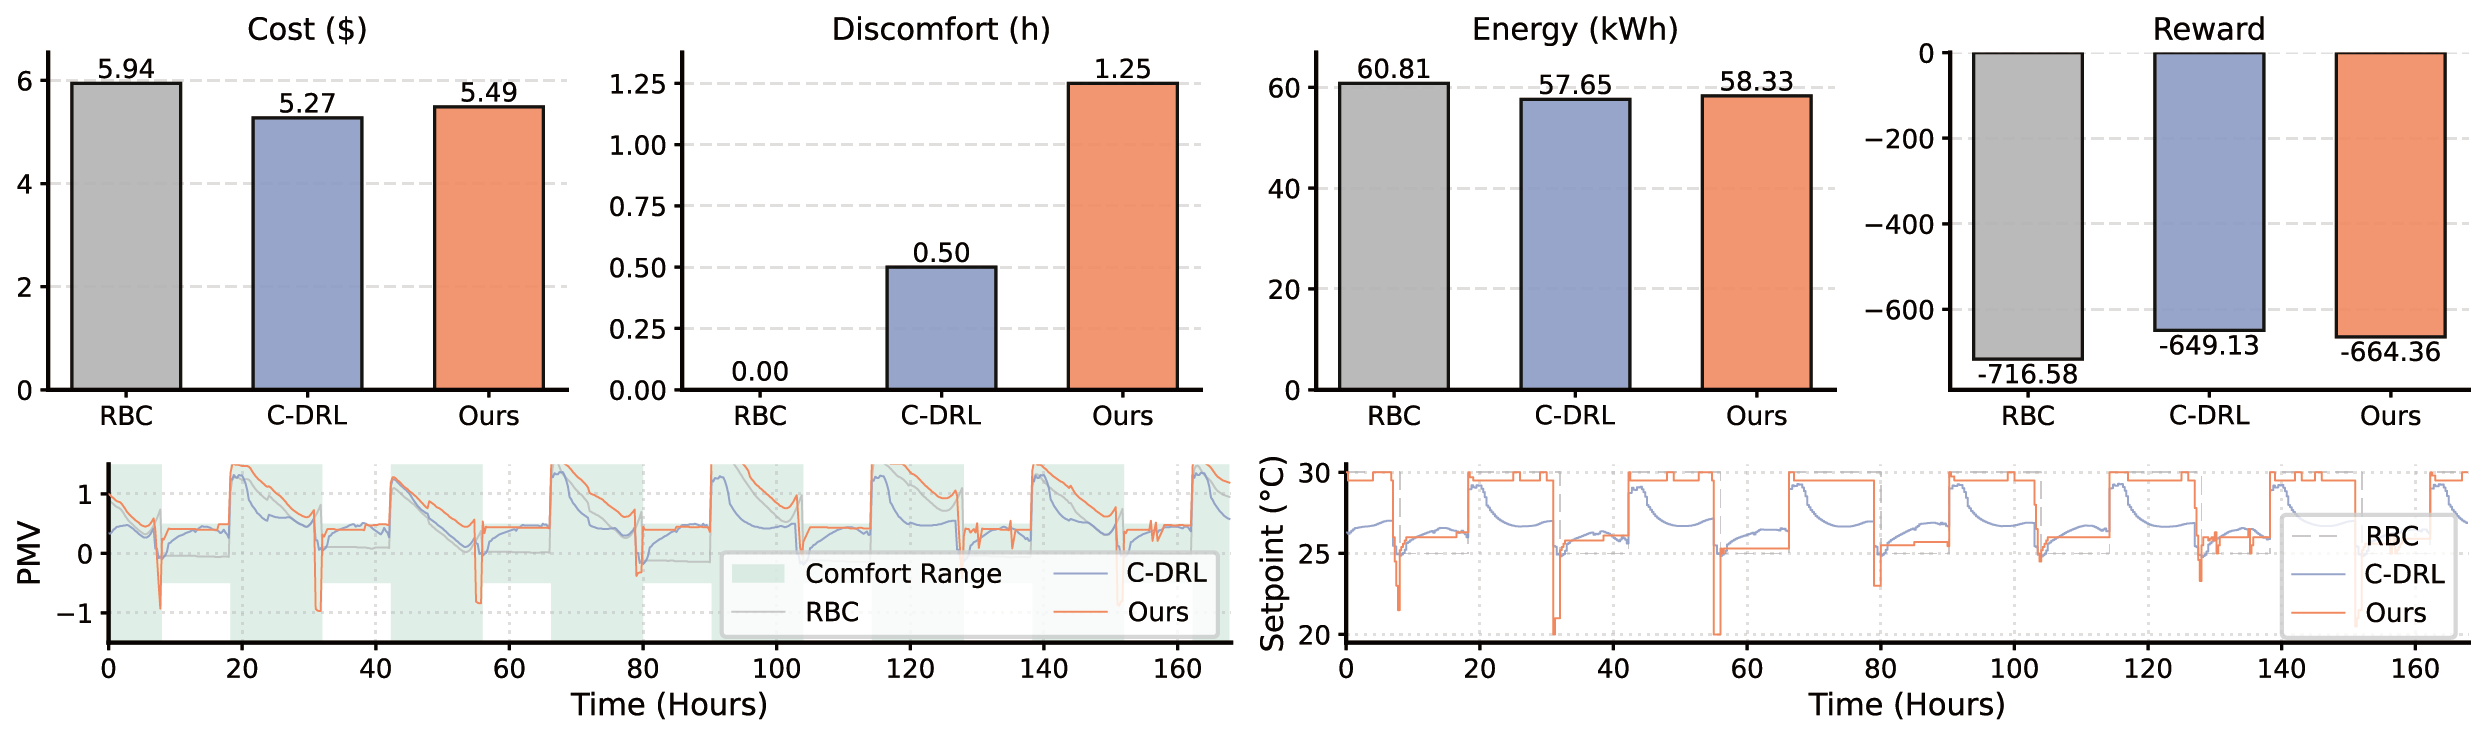
\includegraphics[width=\textwidth]{figs2/Figure_SZ_AIR.png}
    \caption{Performance comparison and control behavior for the \texttt{SZ\_Air} case: (a) cost, energy, and discomfort metrics; (b) setpoint trajectories.}
    \label{fig:sz_air}
\end{figure}

The setpoint trajectories in Fig.~\ref{fig:sz_air}(b) reveal behavioral differences between the two strategies. Both exhibit similar temporal patterns (e.g., pre-cooling during unoccupied periods). However, due to the emphasis on pre-cooling in the safety constraints (Section~3.2.2), the proposed framework's pre-cooling adjustments are more aggressive than those of C-DRL. The key difference manifests during occupied periods: C-DRL performs smooth, continuous fine-tuning throughout the occupancy window, whereas the proposed framework makes only a few discrete adjustments per day. This contrast illustrates DRL's advantage in fine-grained numerical optimization---its continuous policy can fine-tune the setpoint at every 15-minute step, theoretically approaching optimal control more closely. Overall, this case establishes the performance lower bound of the proposed framework in a scenario ideal for DRL (low-dimensional state space, adequate training data, no multi-zone coordination challenges). Nevertheless, given that the framework requires no operational training data, it demonstrates application potential even in this single-zone scenario where its advantages are not fully realized.

\subsubsection{Multi-zone hydronic case (MZ\_Hydro)}

Fig.~\ref{fig:mz_hydro} presents the evaluation results for the \texttt{MZ\_Hydro} case. In this dual-zone FCU hydronic system, the proposed framework achieved the best performance across all evaluation metrics: 42.14\% cost savings over RBC (\$102.63 vs.\ \$177.38), total energy consumption reduced to 801.03~kWh (RBC: 1151.68~kWh), and discomfort duration of only 0.25 zone-hours.

\begin{figure}[pos=!h]
    \centering
    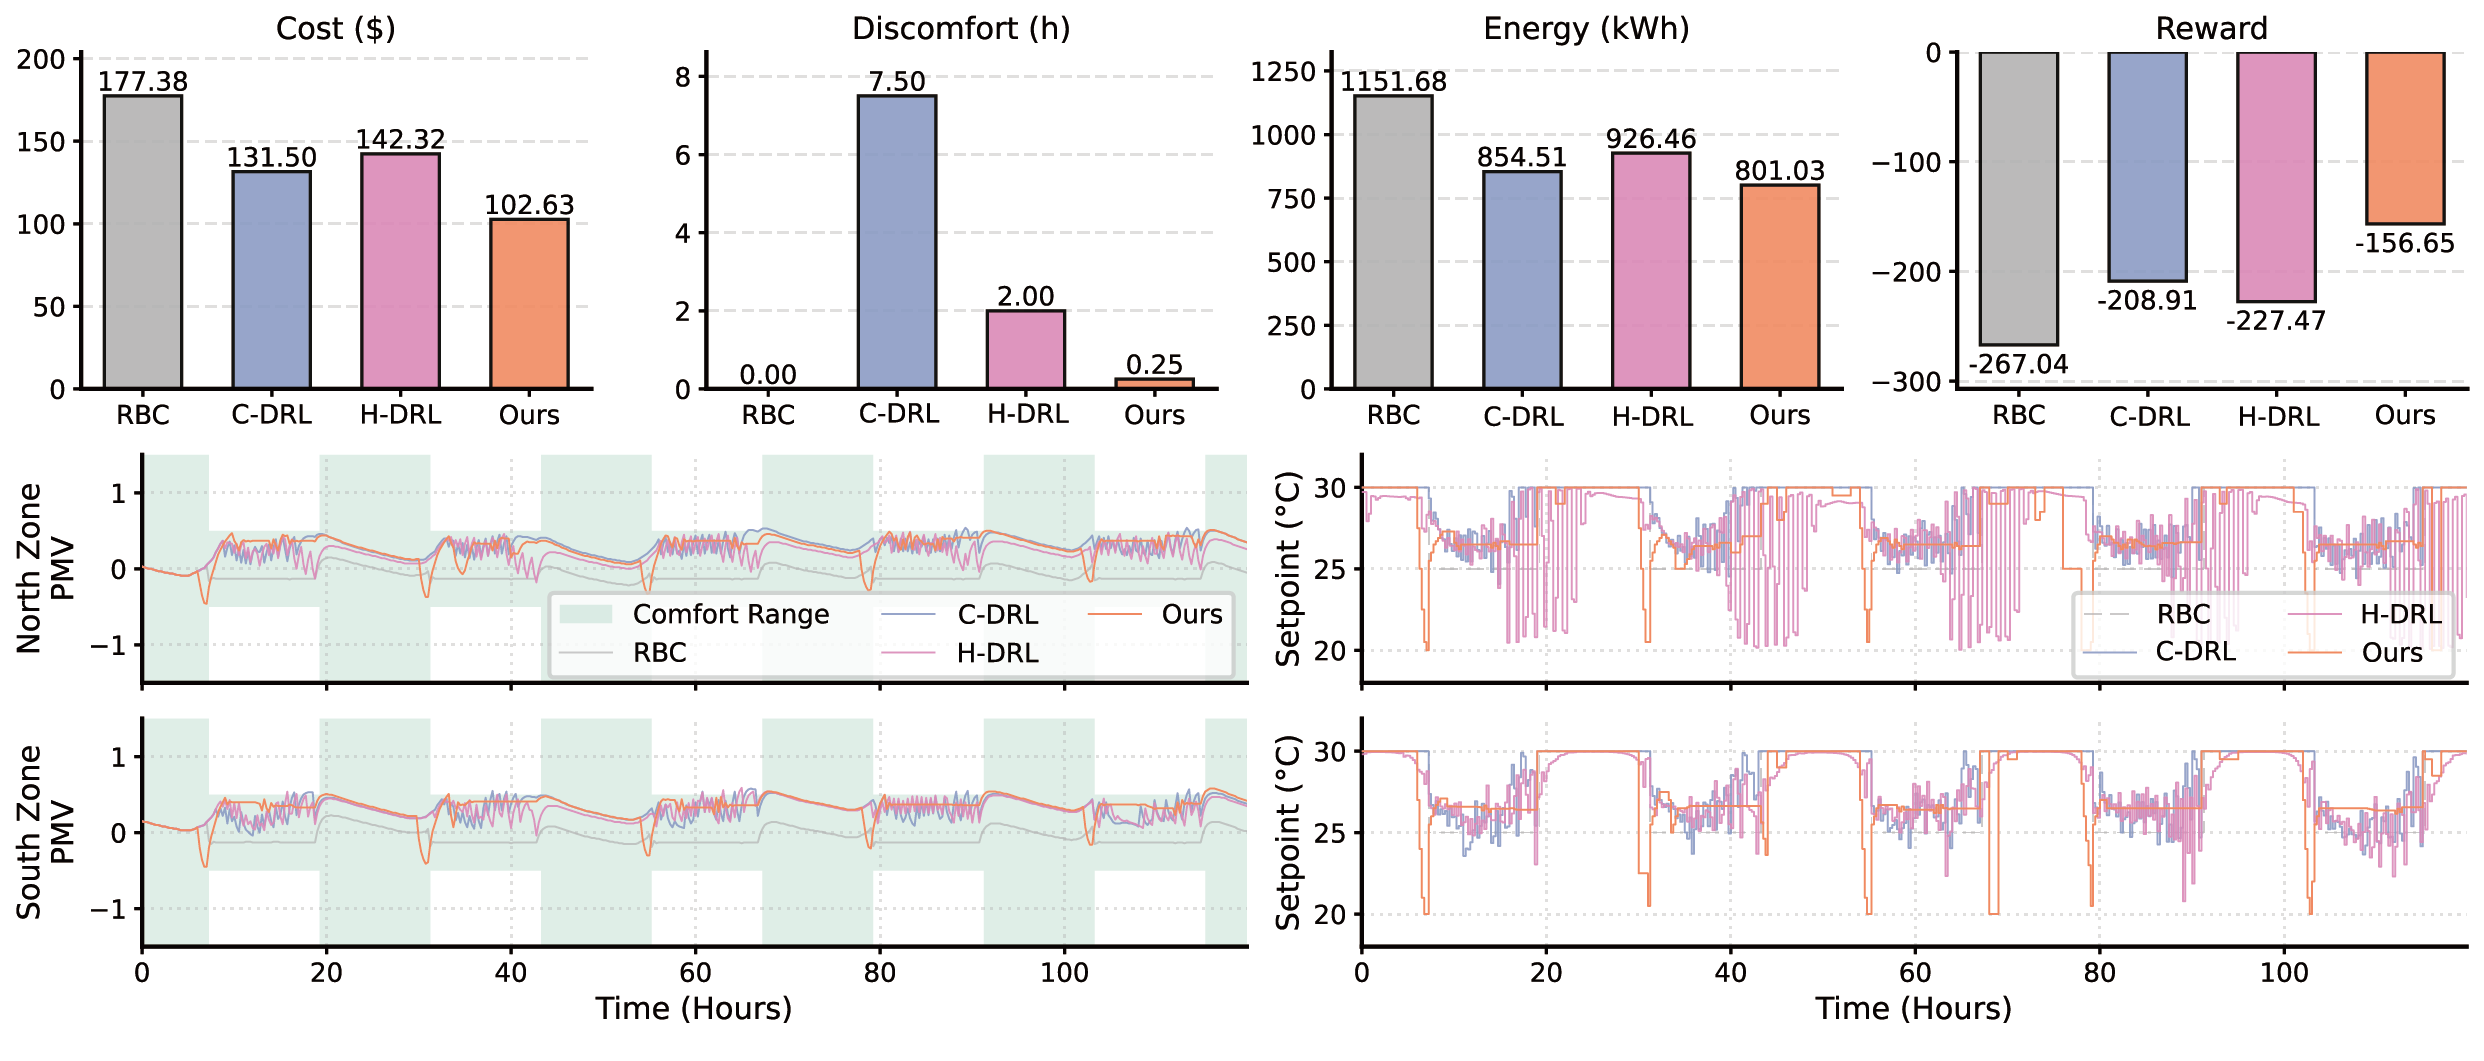
\includegraphics[width=\textwidth]{figs2/Figure_MZ_Hydro.png}
    \caption{Evaluation results for the \texttt{MZ\_Hydro} case: (a) cost, energy, and discomfort metrics; (b) setpoint trajectories for both zones.}
    \label{fig:mz_hydro}
\end{figure}

The performance gap between the two DRL baselines reveals the trade-off between centralized and hierarchical architectures. C-DRL achieved 25.87\% cost savings (\$131.50), exceeding H-DRL's 19.77\% (\$142.32), indicating that in this low-dimensional dual-zone scenario, centralized optimization outperforms decentralized execution in cost efficiency. However, C-DRL's discomfort duration reached 7.50 zone-hours---3.75 times that of H-DRL (2.00 zone-hours). This occurs because the centralized policy sacrifices zone-level comfort in pursuit of global cost optimality, whereas the CTDE architecture's decentralized actors maintain better single-zone comfort awareness under local observations, albeit at the expense of global energy optimization.

The advantage of the proposed framework is visually evident in the setpoint trajectories. As shown in Fig.~\ref{fig:mz_hydro}(b), the framework maintained smooth setpoint trajectories in both zones, while both DRL baselines exhibited oscillatory behavior. H-DRL in particular displayed high-frequency, large-amplitude setpoint adjustments to maintain local comfort, resulting in energy waste. This difference is likely related to the high thermal inertia of the hydronic system and the limited prediction horizon; the underlying mechanism is discussed in Section~\ref{sec:discussion}.

\subsubsection{Multi-zone all-air case (MZ\_Air)}

Fig.~\ref{fig:mz_air} presents the evaluation results for the five-zone VAV all-air system (\texttt{MZ\_Air}). For cost savings relative to RBC, H-DRL achieved the highest (21.60\%, \$141.39), while the proposed framework (16.13\%, \$151.27) fell between C-DRL (15.17\%, \$153.00) and H-DRL. However, in thermal comfort, the proposed framework performed best: discomfort duration was reduced to 13.25 zone-hours, a 22--25\% reduction compared with both DRL baselines (C-DRL: 17.00, H-DRL: 17.75).

\begin{figure}[pos=!h]
    \centering
    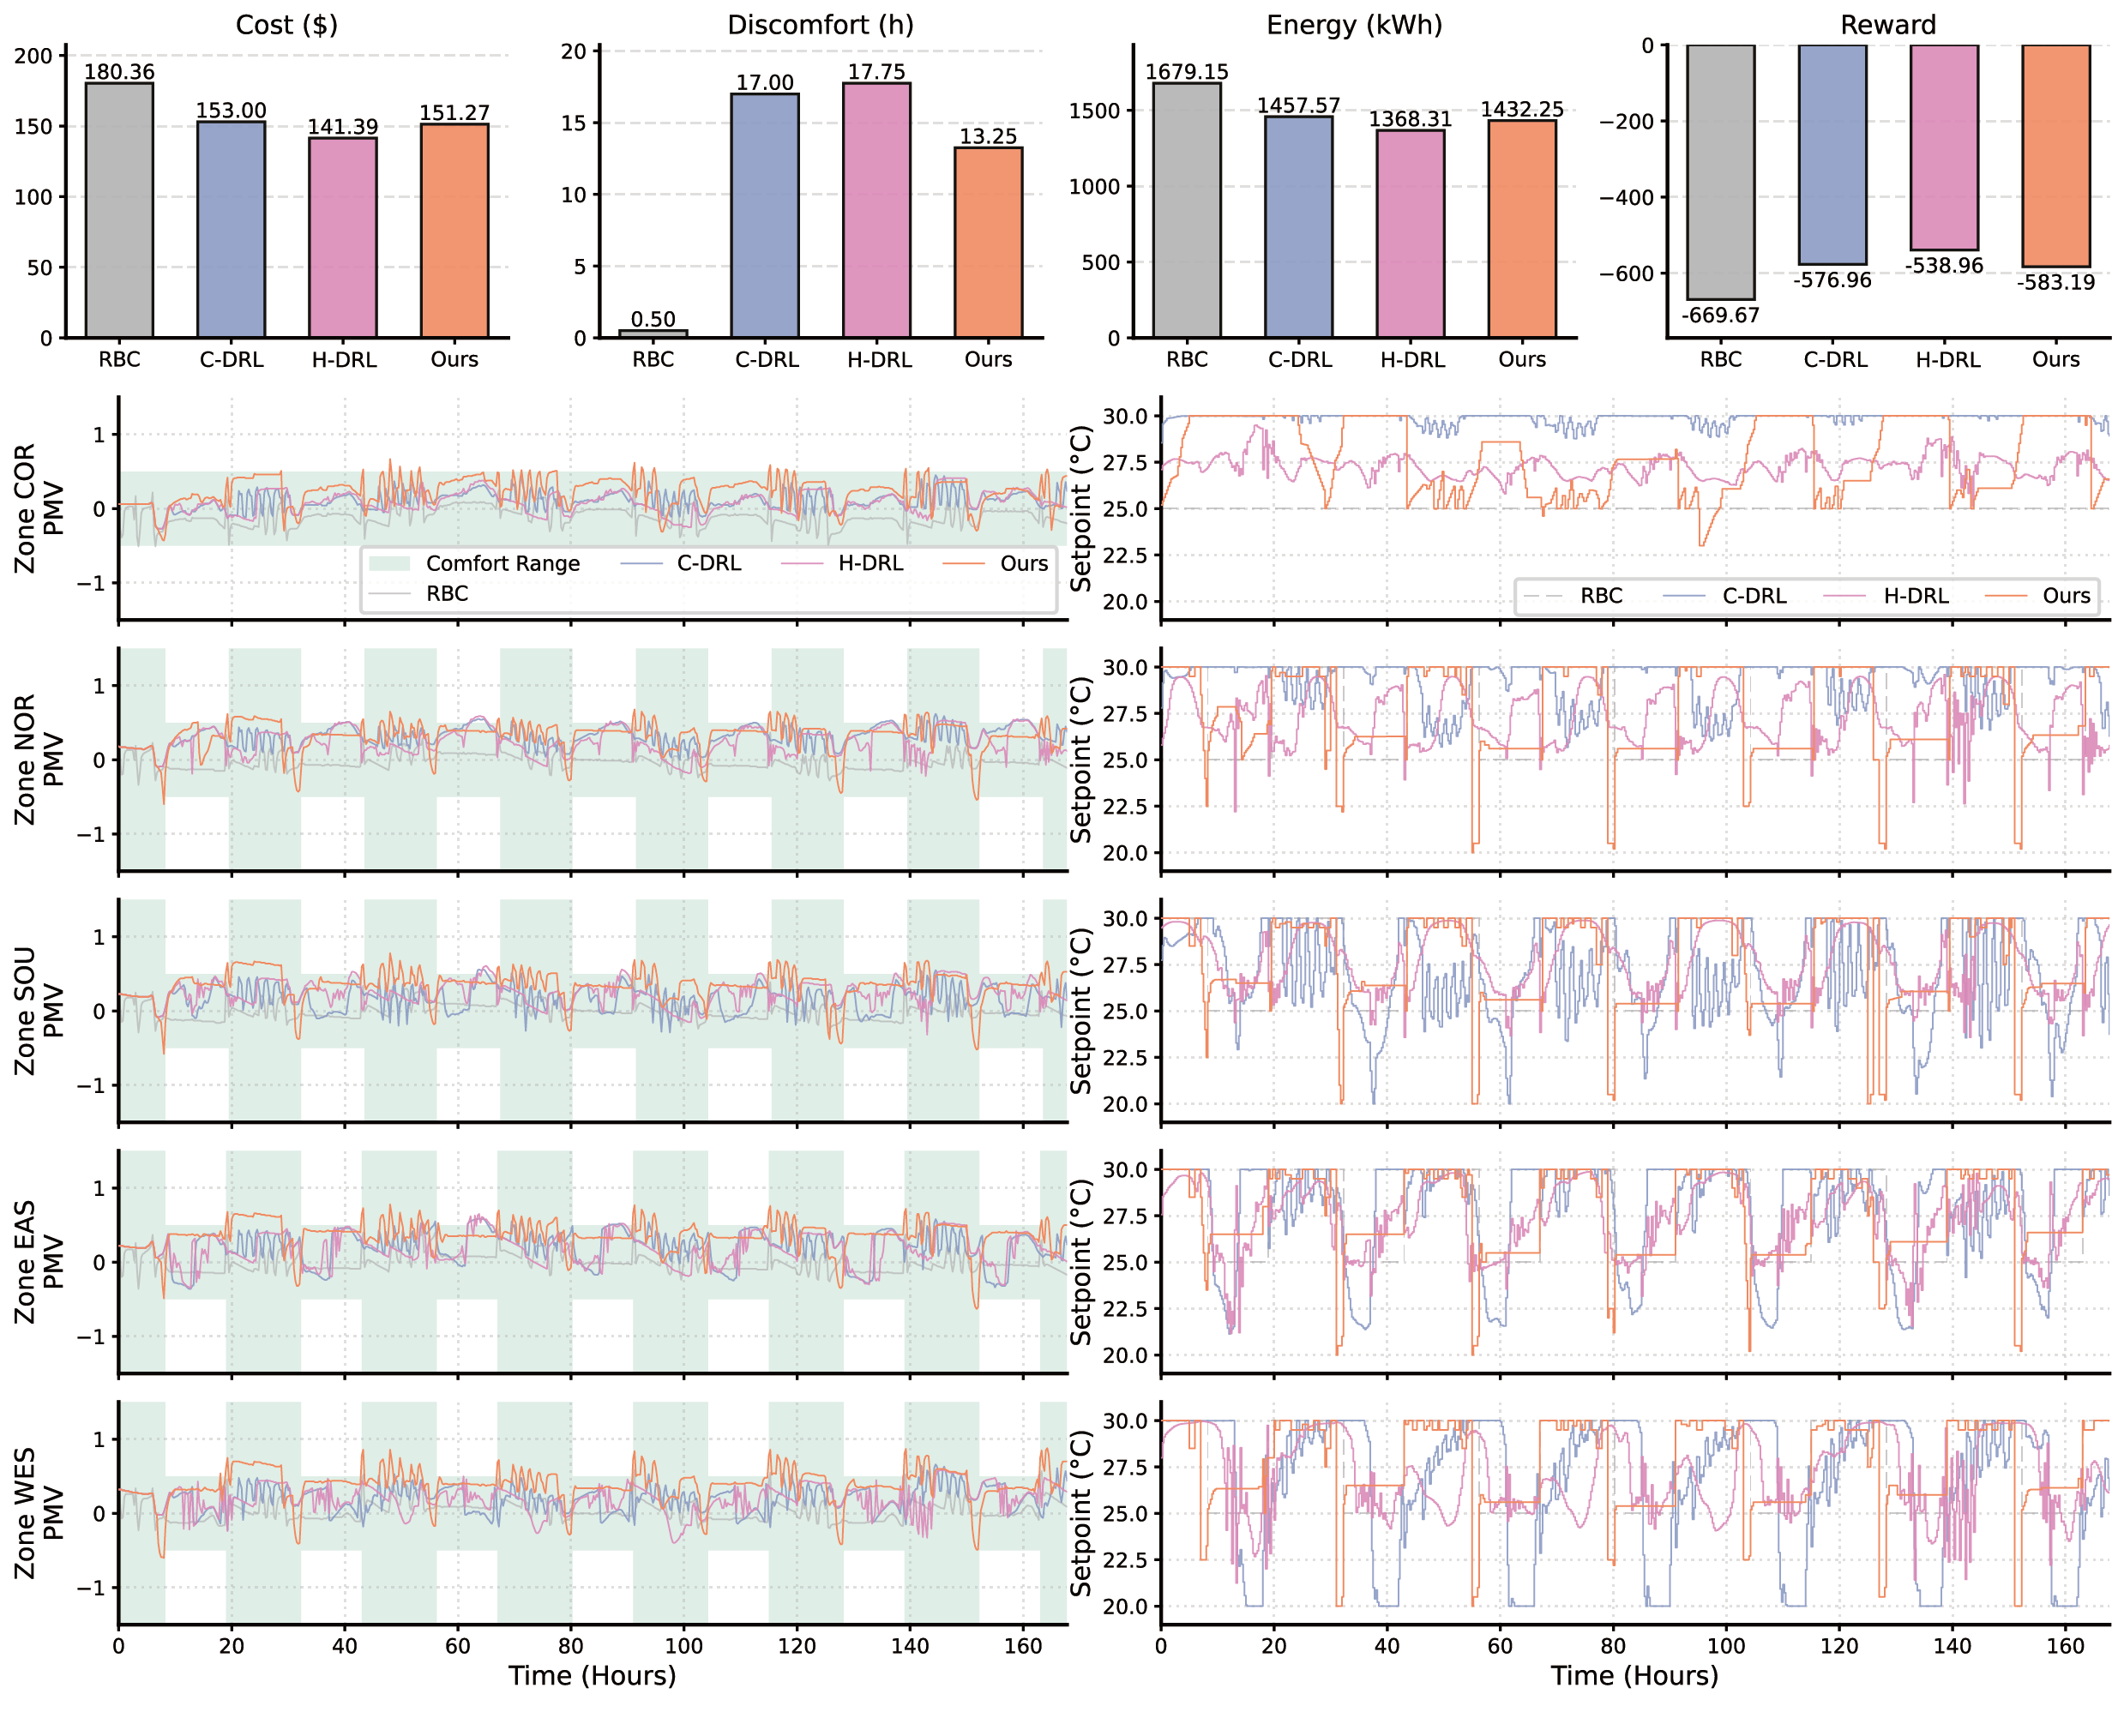
\includegraphics[width=\textwidth]{figs2/Figure_MZ_AIR.png}
    \caption{Evaluation results for the \texttt{MZ\_Air} five-zone case: (a) cost, energy, and discomfort metrics; (b) setpoint trajectories for all five zones.}
    \label{fig:mz_air}
\end{figure}

The performance reversal between H-DRL and C-DRL in the \texttt{MZ\_Air} case compared with \texttt{MZ\_Hydro} corroborates the scalability bottleneck of centralized architectures in multi-agent learning. As the five-zone joint action space expands to $[20, 30]^5$, the single PPO policy's representational capacity becomes insufficient for fine-grained five-zone coordination; the MAPPO architecture in H-DRL, through its combination of distributed actors and a centralized critic, effectively mitigates this high-dimensional control challenge.

Further temporal analysis in Fig.~\ref{fig:mz_air}(b) reveals the control logic and trade-off boundaries of each strategy. H-DRL achieves near-optimal control in the high-dimensional setting through continuous fine-tuning across all time periods (e.g., aggressive nighttime pre-cooling and daytime high-frequency fluctuations) to track cross-zone thermal coupling dynamics. In contrast, C-DRL's control curves exhibit pronounced oscillations, exposing the representational limitations of centralized policy networks in high-dimensional settings---a factor that also explains its higher energy expenditure. The proposed approach instead generates control actions based on causal relationships and semantic reasoning, producing low-frequency but more stable actions that balance safety, stability, and optimality. Notably, for the COR zone---where thermal coupling effects are strongest---the proposed framework produced a control pattern similar to H-DRL, in contrast to C-DRL's nearly constant 30\,$^{\circ}$C setpoint. This suggests that semantic reasoning can identify control patterns comparable to those of data-driven methods.


\subsection{Causal augmentation mechanism analysis}

To quantify the effect of causal augmentation on Orchestrator reasoning quality, we conducted an ablation experiment. With all other framework components held constant, the framework was run under two configurations: with causal rule injection (Causal) and without (Baseline). Decision reliability was evaluated using the three agent behavior audit metrics defined in Section~3: hallucination rate $R_H$ (Eq.~(\ref{eq:hallucination})), semantic jitter $J$ (Eq.~(\ref{eq:jitter})), and safety intervention rate $R_{\text{SIR}}$ (Eq.~(\ref{eq:sir})). Fig.~\ref{fig:causal} presents the ablation results.


Changes in hallucination rate most directly reflect the effect of causal rules on reasoning quality. In \texttt{SZ\_Air}, $R_H$ decreased from 56.6\% to 7.7\% (86.3\% reduction); in \texttt{MZ\_Hydro}, from 57.9\% to 12.9\% (77.7\% reduction). This indicates that without causal rules, the Orchestrator's reasoning contradicted the actual physical state in more than half of all time steps. After causal rule injection, hallucination rates dropped sharply; the residual 7--13\% primarily stems from the inherent uncertainty of LLM probabilistic reasoning (e.g., format deviations), while systematic physical misjudgments were effectively suppressed. \texttt{MZ\_Air} exhibited a different pattern: the baseline hallucination rate was only 19.4\%, and causal rules further reduced it to 16.0\% (17.8\% reduction). The differential reduction across cases is discussed in Section~\ref{sec:discussion}.

The change in safety intervention rate was the most dramatic among the three metrics. Causal augmentation nearly eliminated safety interventions across all cases: \texttt{SZ\_Air} decreased from 51.2\% to 0.6\% (98.8\% reduction), \texttt{MZ\_Hydro} from 30.4\% to 0.4\% (98.6\% reduction), and \texttt{MZ\_Air} from 1.1\% to 0.0\% (100\% reduction). Without causal rules, the Orchestrator frequently issued directives contradicting physical constraints (e.g., requesting large setpoint jumps in high-inertia systems), forcing the Executor layer's safety mechanism to apply corrective overrides. With causal rules, the Orchestrator's directives were physically compatible at the source, demoting the safety layer from a frequently invoked error-correction mechanism to a redundant safeguard. This demonstrates that causal augmentation achieves proactive safety alignment rather than reactive safety correction.

The setpoint change magnitude distributions in Fig.~\ref{fig:causal}(a) further reveal the behavioral mechanism of causal augmentation. Across all cases, injecting causal rules shifted the distribution of setpoint adjustments ($|\Delta\text{SP}|$) toward smaller magnitudes, with this trend most pronounced in \texttt{MZ\_Hydro}. This shift indicates that causal rules constrain the Orchestrator to produce moderate, physically grounded strategies rather than aggressive step changes, which in turn explains the decline in safety intervention rate.

\begin{figure}[pos=t]
    \centering
    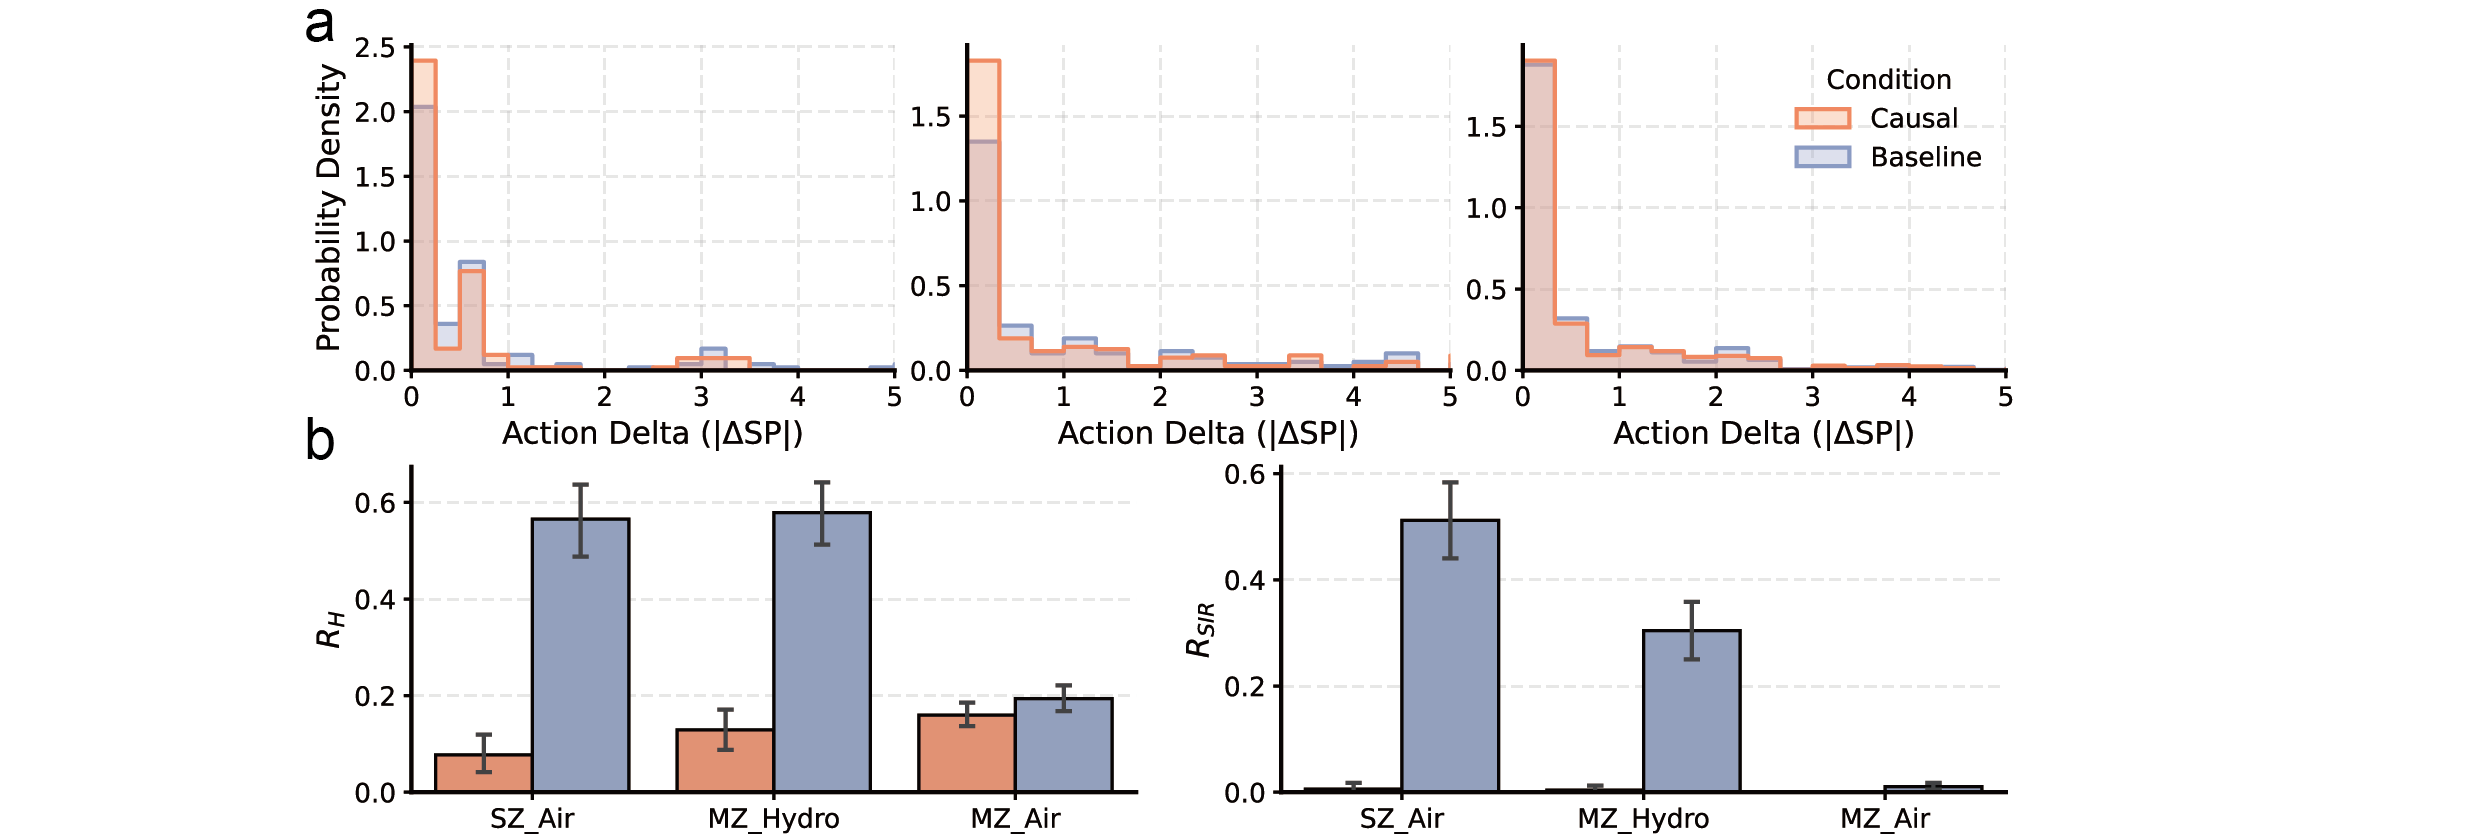
\includegraphics[width=\textwidth]{figs2/Figure_Causal.png}
    \caption{Causal augmentation ablation results: hallucination rate, safety intervention rate, and setpoint change distributions with and without causal rules across three cases.}
    \label{fig:causal}
\end{figure}

In summary, the core contribution of causal augmentation extends beyond competitive control performance (already measured by physical metrics in Section~5.1) to establishing a trustworthy reasoning foundation. The substantial reduction in $R_H$ and near-elimination of $R_{\text{SIR}}$ indicate that the framework's control decisions are grounded in physical reality rather than merely probabilistic predictions---a necessary precondition for deploying LLM-based controllers in real building environments.

\subsection{Working memory window analysis}

This ablation experiment determines the optimal memory depth $k$ by varying it from 0 (no memory, fully stateless) to 3 (three-hour lookback), with all other configurations held constant. Memory depth is evaluated across three dimensions: total reward, semantic jitter $J$, and input token count.


The reward analysis in Fig.~\ref{fig:sw_ablation}(a) reveals an inverted U-shaped curve consistent across all three cases. In all cases, $k=1$ was the optimal configuration: \texttt{SZ\_Air} per-zone reward improved from $-673.89$ at $k=0$ to $-664.39$ at $k=1$ (1.4\% improvement), \texttt{MZ\_Hydro} from $-162.50$ to $-156.68$ (3.6\%), and \texttt{MZ\_Air} from $-593.68$ to $-583.19$ (1.8\%). However, performance at $k=2$ and $k=3$ degraded, approaching or falling back to $k=0$ levels. This inverted U-shaped curve reflects a trade-off between information and noise: a one-hour lookback provides the minimum viable context for closed-loop temporal reasoning, while additional memory introduces redundant signals that dilute decision-relevant information density.

\begin{figure}[pos=t]
    \centering
    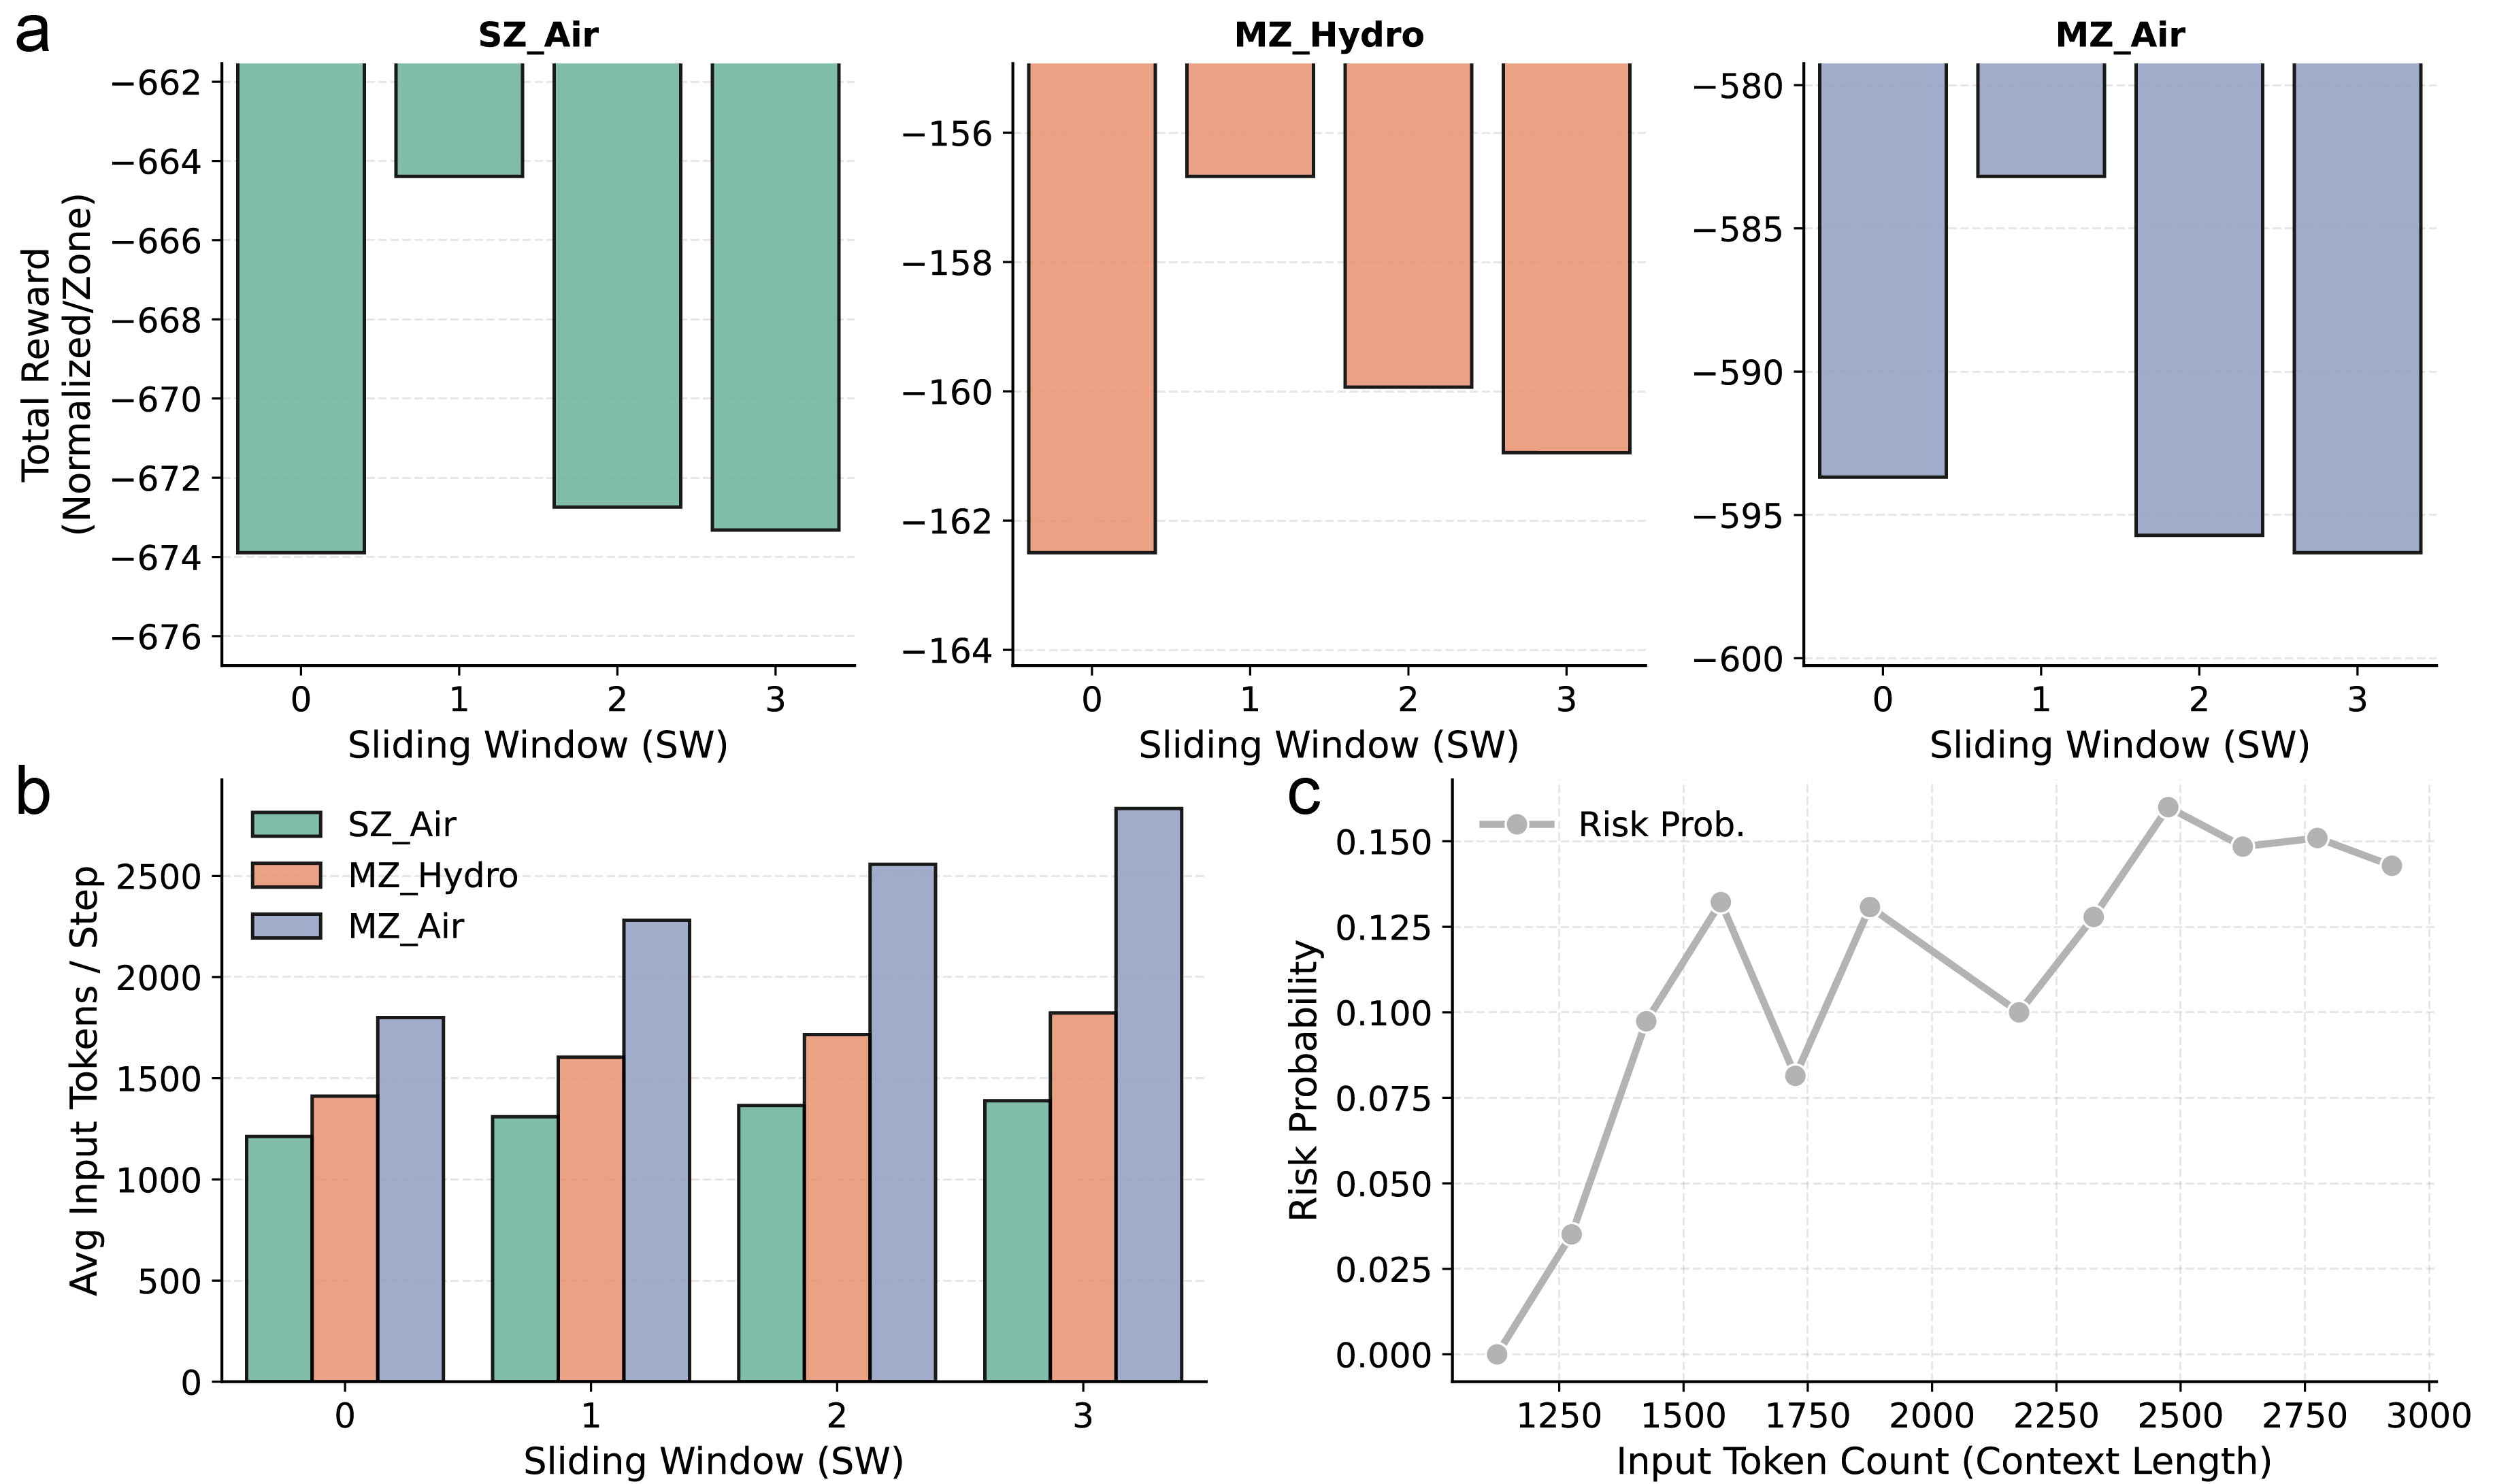
\includegraphics[width=0.7\textwidth]{figs2/Figure_SW_Ablation.png}
    \caption{Working memory window ablation: (a) per-zone reward as a function of $k$; (b) input token counts; (c) context risk probability.}
    \label{fig:sw_ablation}
\end{figure}

\begin{figure}[pos=t]
    \centering
    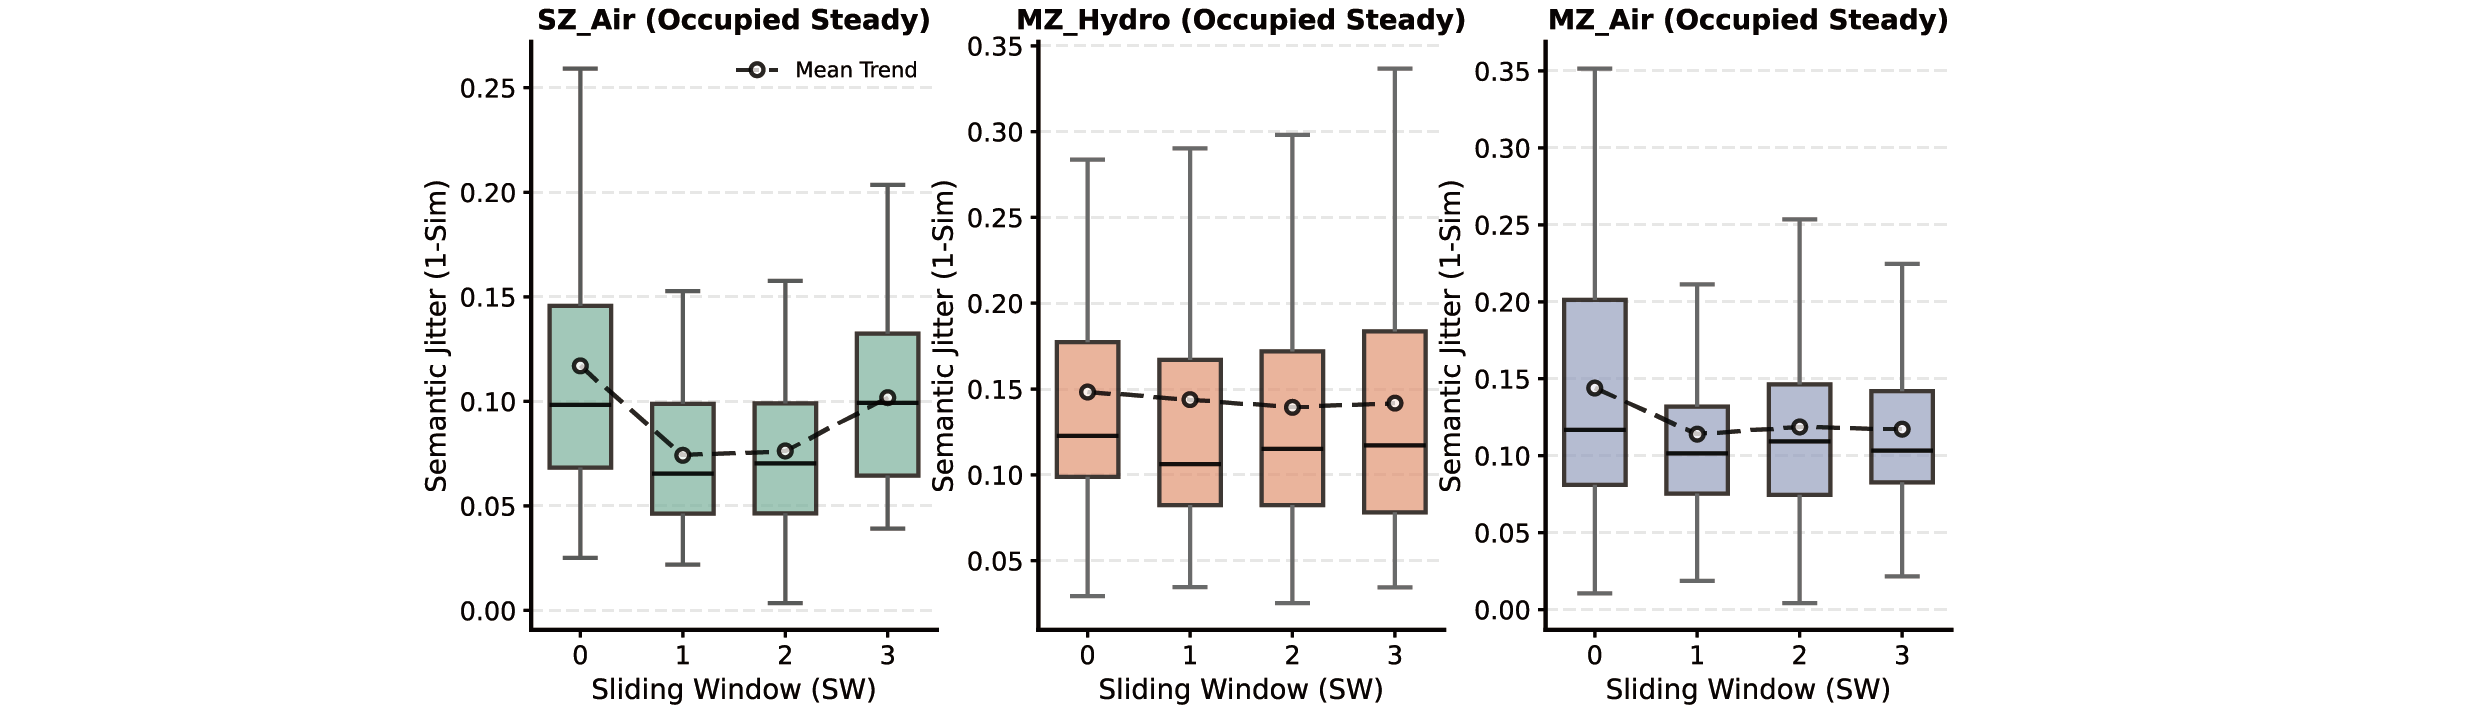
\includegraphics[width=\textwidth]{figs2/Figure_Stability.png}
    \caption{Semantic jitter analysis under steady-state occupancy conditions as a function of memory window $k$.}
    \label{fig:stability}
\end{figure}

The semantic jitter analysis in Fig.~\ref{fig:stability} validates these findings from a decision stability perspective. Under steady-state occupancy conditions, \texttt{SZ\_Air} exhibits a clear U-shaped jitter curve ($J$ decreased from 0.117 at $k=0$ to 0.074 at $k=1$, 0.076 at $k=2$, then rose to 0.102 at $k=3$). \texttt{MZ\_Air} shows a pronounced drop from $k=0$ to $k=1$ (0.144 to 0.114), then stabilizes. These patterns indicate that without memory, each Orchestrator decision is independent, and adjacent directives may contradict each other, resulting in high semantic jitter. A single hour of context ($k=1$) provides sufficient information to stabilize the reasoning chain. Beyond $k=1$, jitter reduction saturates or reverses, consistent with the reward degradation trend. The jitter curve for \texttt{MZ\_Hydro} is relatively flat (ranging from 0.148 to 0.139).

The context risk curve in Fig.~\ref{fig:sw_ablation}(c) provides a mechanistic explanation for the inverted U-shaped phenomenon. Risk probability increases monotonically from approximately 0\% at ${\sim}$1125 tokens to approximately 15\% above 2500 tokens. Each additional memory entry adds approximately 100--250 input tokens. In the $k=1$ range of approximately 1300--1600 tokens, risk probability remains at 3--9\%. In the $k=3$ range of approximately 1400--2800 tokens, risk probability rises to 10--15\%. The marginal information gain from older memories cannot compensate for this increasing error probability. The consistent optimality of $k=1$ across three substantially different cases suggests that this is a robust configuration for building control at the 15-minute/hourly decision interval.

% === SECTION 6: Discussion === %
\section{Discussion}
\label{sec:discussion}

\subsection{Research significance}

To the best of our knowledge, this study provides the first systematic empirical comparison of a hierarchical LM-MA framework against DRL baselines across heterogeneous building types. The proposed framework achieved competitive cost savings relative to fully trained DRL baselines without environment interaction training, and attained the best overall performance among all methods in the dual-zone hydronic case.

Synthesizing results across the three cases, several findings emerge. First, no single DRL architecture dominates across all building scales: C-DRL outperformed H-DRL in the low-dimensional setting (dual-zone), while H-DRL surpassed C-DRL in the high-dimensional setting (five-zone). This scale-dependent performance reversal reflects a practical engineering challenge---architectural selection requires scenario-specific adaptation. Second, the core advantages of the proposed framework lie not in numerical optimization but in three dimensions: (a)~zero-shot deployment capability---the same framework adapts to three heterogeneous configurations by replacing only the offline causal rules; (b)~consistent comfort assurance across system types---whereas DRL baselines tend to sacrifice comfort for cost optimization, the proposed framework maintained the most consistent comfort performance across all three cases; and (c)~strongest performance in thermally inertia-dominated scenarios (e.g., hydronic systems), where causal augmentation provides the greatest marginal value.

The framework's pronounced advantage in hydronic systems stems from its resolution of the mismatch between prediction horizon and response delay in high-thermal-inertia systems. The thermal response delay of hydronic systems exceeds the available one-hour weather forecast horizon, creating a credit assignment problem for DRL policies that promotes overfitting to short-term meteorological fluctuations and control oscillations. The high discomfort duration of C-DRL in this case is consistent with this interpretation. In contrast, the proposed framework explicitly encodes inertia awareness and pre-cooling strategies through causal rules, enabling the Orchestrator to generate policies matched to physical time scales without data fitting. This result suggests that when system dynamics operate on time scales exceeding the available prediction horizon, semantic reasoning may offer greater marginal value relative to data-driven fitting.

In all-air systems, DRL baselines achieved higher cost savings, likely because the minute-scale thermal response closely matches the DRL execution step. However, even at a cost disadvantage, the framework achieved the best comfort performance in the five-zone case and exhibited control patterns similar to H-DRL in the zone with the strongest thermal coupling. The substantially lower baseline hallucination rate in \texttt{MZ\_Air} compared with the other two cases may reflect richer VAV/AHU knowledge in LLM pre-training corpora, leaving less room for marginal improvement via causal rules. Across both system types, the framework's applicability boundaries emerge: its engineering value is most pronounced where system inertia renders data-driven fitting unreliable and where comfort assurance takes priority over marginal cost optimization.

Ablation experiments demonstrated that causal rules function as physical inductive biases, narrowing the LLM's output distribution from a broad probability space to the thermodynamically feasible subspace. The differential effects across cases may stem from uneven LLM pre-training coverage across system types, with causal rules providing greater marginal contribution for hydronic systems that appear less frequently in general corpora. The near-elimination of safety interventions suggests a proactive safety alignment mode---Orchestrator directives are physically compatible at the point of generation, demoting the safety layer from a frequently invoked corrector to a redundant safeguard. Unlike multi-round self-correction frameworks and retrieval-augmented generation, causal rules are static, zero-runtime-overhead structural constraints that bound outputs at the reasoning logic level. Nevertheless, the residual hallucination rate confirms that deterministic safety layers remain necessary.

The consistent optimality of $k=1$ across all cases yields a design principle for LLM-based real-time control: context should be minimized to decision-critical information rather than maximizing information completeness. A one-hour lookback provides the minimum viable context for closed-loop reasoning; additional memory dilutes decision-relevant information density and elevates context risk. The U-shaped semantic jitter curve in \texttt{SZ\_Air} corroborates this: excess memory introduces contradictory signals that destabilize the reasoning chain. The relatively flat jitter curve in \texttt{MZ\_Hydro} reflects the interaction between thermal inertia and causal rules---high thermal inertia smooths context differences across memory lengths, while inertia-aware information encoded in causal rules reduces the model's dependence on historical context. The robustness of $k=1$ across three substantially different cases provides initial support for this design principle in building control.

These findings suggest that the combination of semantic reasoning and physical causal priors constitutes a viable control paradigm that exists alongside---rather than replacing---physics-based and data-driven methods. Its core principle is separation of concerns: causal knowledge provides inductive biases, semantic reasoning handles multi-zone coordination, and deterministic constraints ensure safety. At the practical level, framework deployment requires only building technical documentation rather than months of operational data collection, directly addressing the reality that many existing buildings lack data infrastructure. Synthesizing cross-case results, the framework is most applicable to high-inertia building systems, existing buildings with limited BMS data, and application environments with stringent comfort compliance requirements.

\subsection{Limitations and future work}

Despite competitive zero-shot control performance across three heterogeneous cases, this study has several limitations. All evaluations were conducted in the BOPTEST simulation environment; real-deployment challenges such as sensor noise, communication latency, and stochastic occupant behavior have not been examined. Causal rules remained static during the evaluation period, an assumption valid for the one-week evaluation window. However, real building operation spans months to years, during which the applicability conditions of causal rules change with seasons and operating conditions; the current framework lacks a dynamic adaptation mechanism. Additionally, causal rule authoring depends on domain expert prior knowledge, shifting the deployment barrier from data collection to knowledge engineering. Furthermore, the framework's dependence on external LLM APIs may limit deployment efficiency and economic feasibility in large-scale building portfolios.

These limitations suggest several directions for future research. Dynamic rule updating mechanisms or season-aware causal rule libraries could extend the framework's scope from week-scale to year-round operation. Methods for automatically extracting causal rules from building information models (BIM) or technical documentation could reduce dependence on expert knowledge. Field deployment in controlled experimental buildings is needed to quantify the simulation-to-reality performance gap. Finally, local deployment of small language models should be evaluated to establish a lifecycle cost--benefit analysis that incorporates inference costs.

% === SECTION 7: Conclusion === %
\section{Conclusion}
\label{sec:conclusion}

This paper proposed a causal-augmented hierarchical control framework that achieves zero-shot HVAC control across heterogeneous buildings by injecting thermodynamic causal priors into a hierarchical multi-agent LLM architecture. Systematic evaluation across three benchmark cases demonstrated that the framework competes with fully trained DRL baselines without environment interaction training. It achieved the best overall performance in the high-inertia hydronic system. The framework's advantages are more pronounced when the characteristic time scale of system dynamics exceeds the available prediction horizon, particularly under stringent comfort requirements. Causal augmentation effectively suppressed reasoning hallucinations and nearly eliminated safety interventions, indicating that structured physical knowledge can improve LLM control reliability. These findings suggest that physical causal priors can serve as a complementary foundation for scalable building control, enabling deployment that relies solely on technical documentation for existing buildings lacking operational data. Future work will focus on online adaptive updating of causal rules and on validating framework performance in real buildings.

\section*{CRediT authorship contribution statement}
\begin{description}
    \item[Weilin Xin:]
    \item[Wei Liang:]
    \item[Adrian Chong:]
\end{description}

\section*{Declaration of Generative AI and AI-assisted technologies in the writing process}
During the preparation of this work the authors used Gemini in order to check grammar and language. After using this tool, the authors reviewed and edited the content as needed and take full responsibility for the content of the publication.

\section*{Declaration of competing interest}
The authors declare that they have no known competing financial interests or personal relationships that could have appeared to influence the work reported in this paper.

\section*{Data accessibility}
The data and code supporting the findings of this study are available at \url{https://github.com/ideas-lab-nus/Causal_augmented_Hierarchical_Control.git}.

\section*{Acknowledgments}

\printcredits

\bibliographystyle{model1-num-names}
\bibliography{improve}

\clearpage
\appendix
\setcounter{figure}{0}
\renewcommand{\thefigure}{A\arabic{figure}}

% === APPENDIX A: Prompt Design === %
\section{Prompt Design}

\begin{figure}[pos=ht]
    \centering
    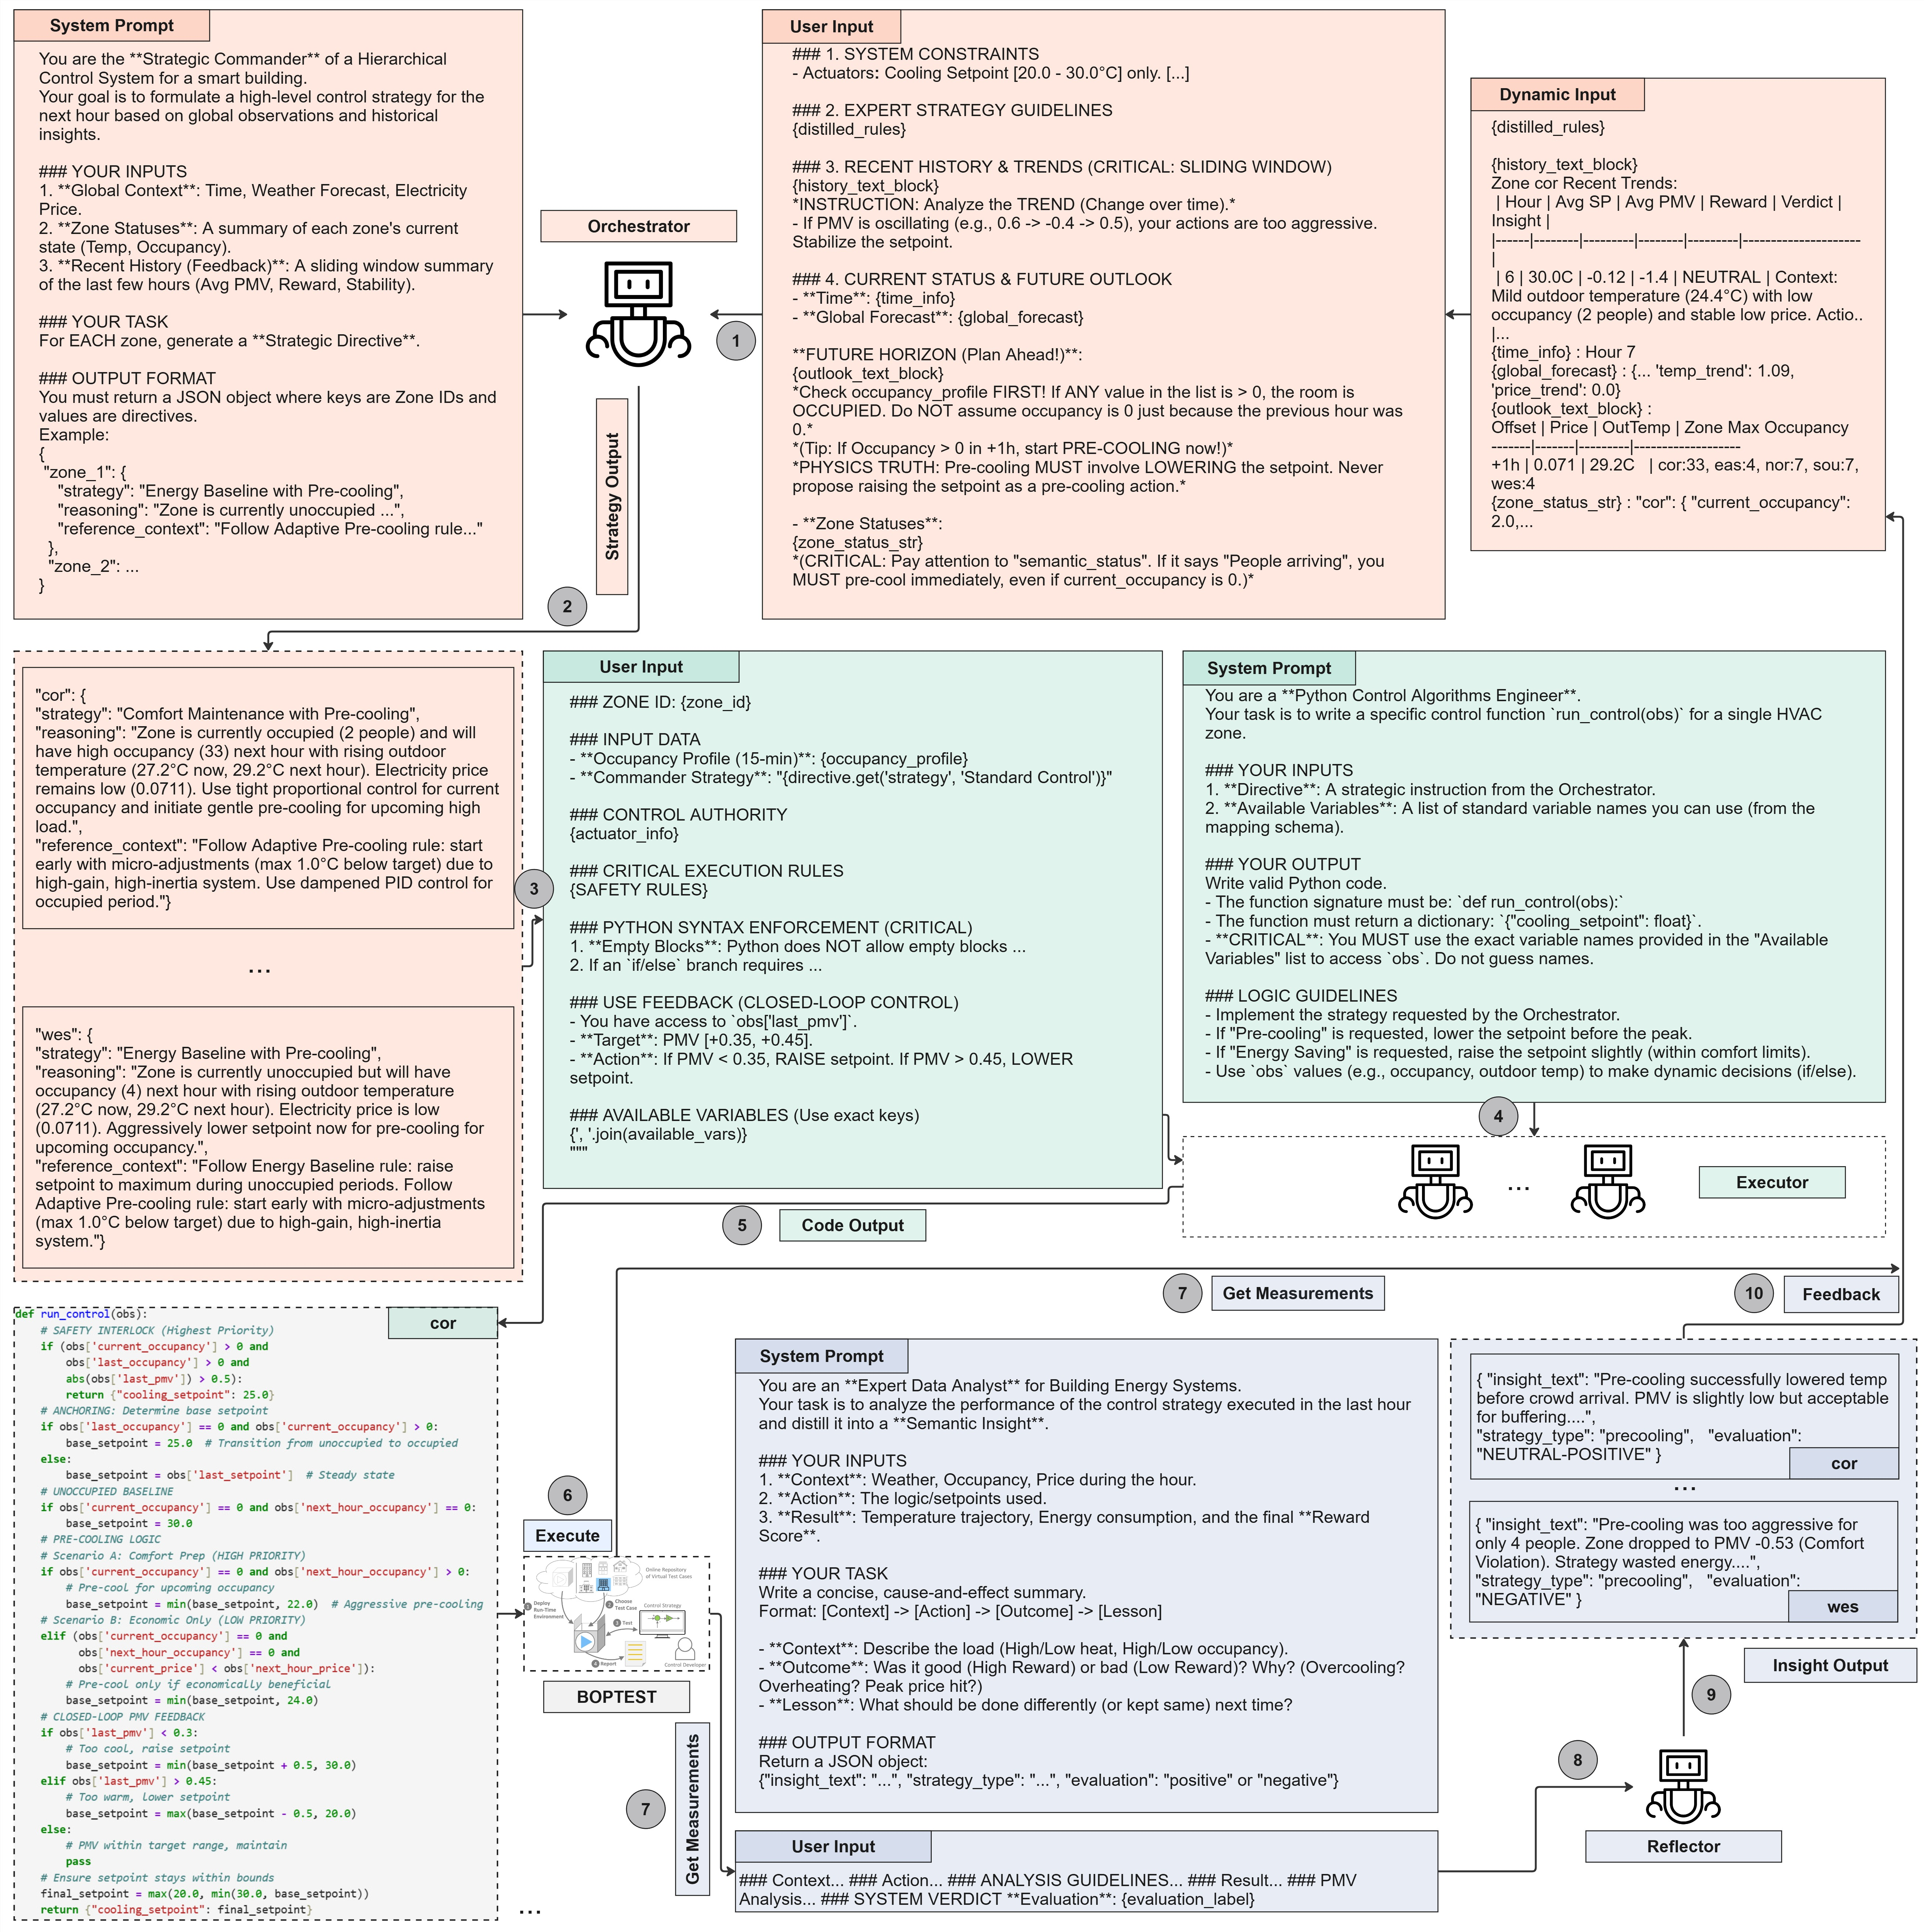
\includegraphics[width=0.7\textwidth]{figs2/CloseLoop_Prompt.jpg}
    \caption{Prompt templates for the Orchestrator, Executor, and Reflector agents in the online control loop.}
    \label{fig:closeloop_prompt}
\end{figure}

\begin{figure}[pos=ht]
    \centering
    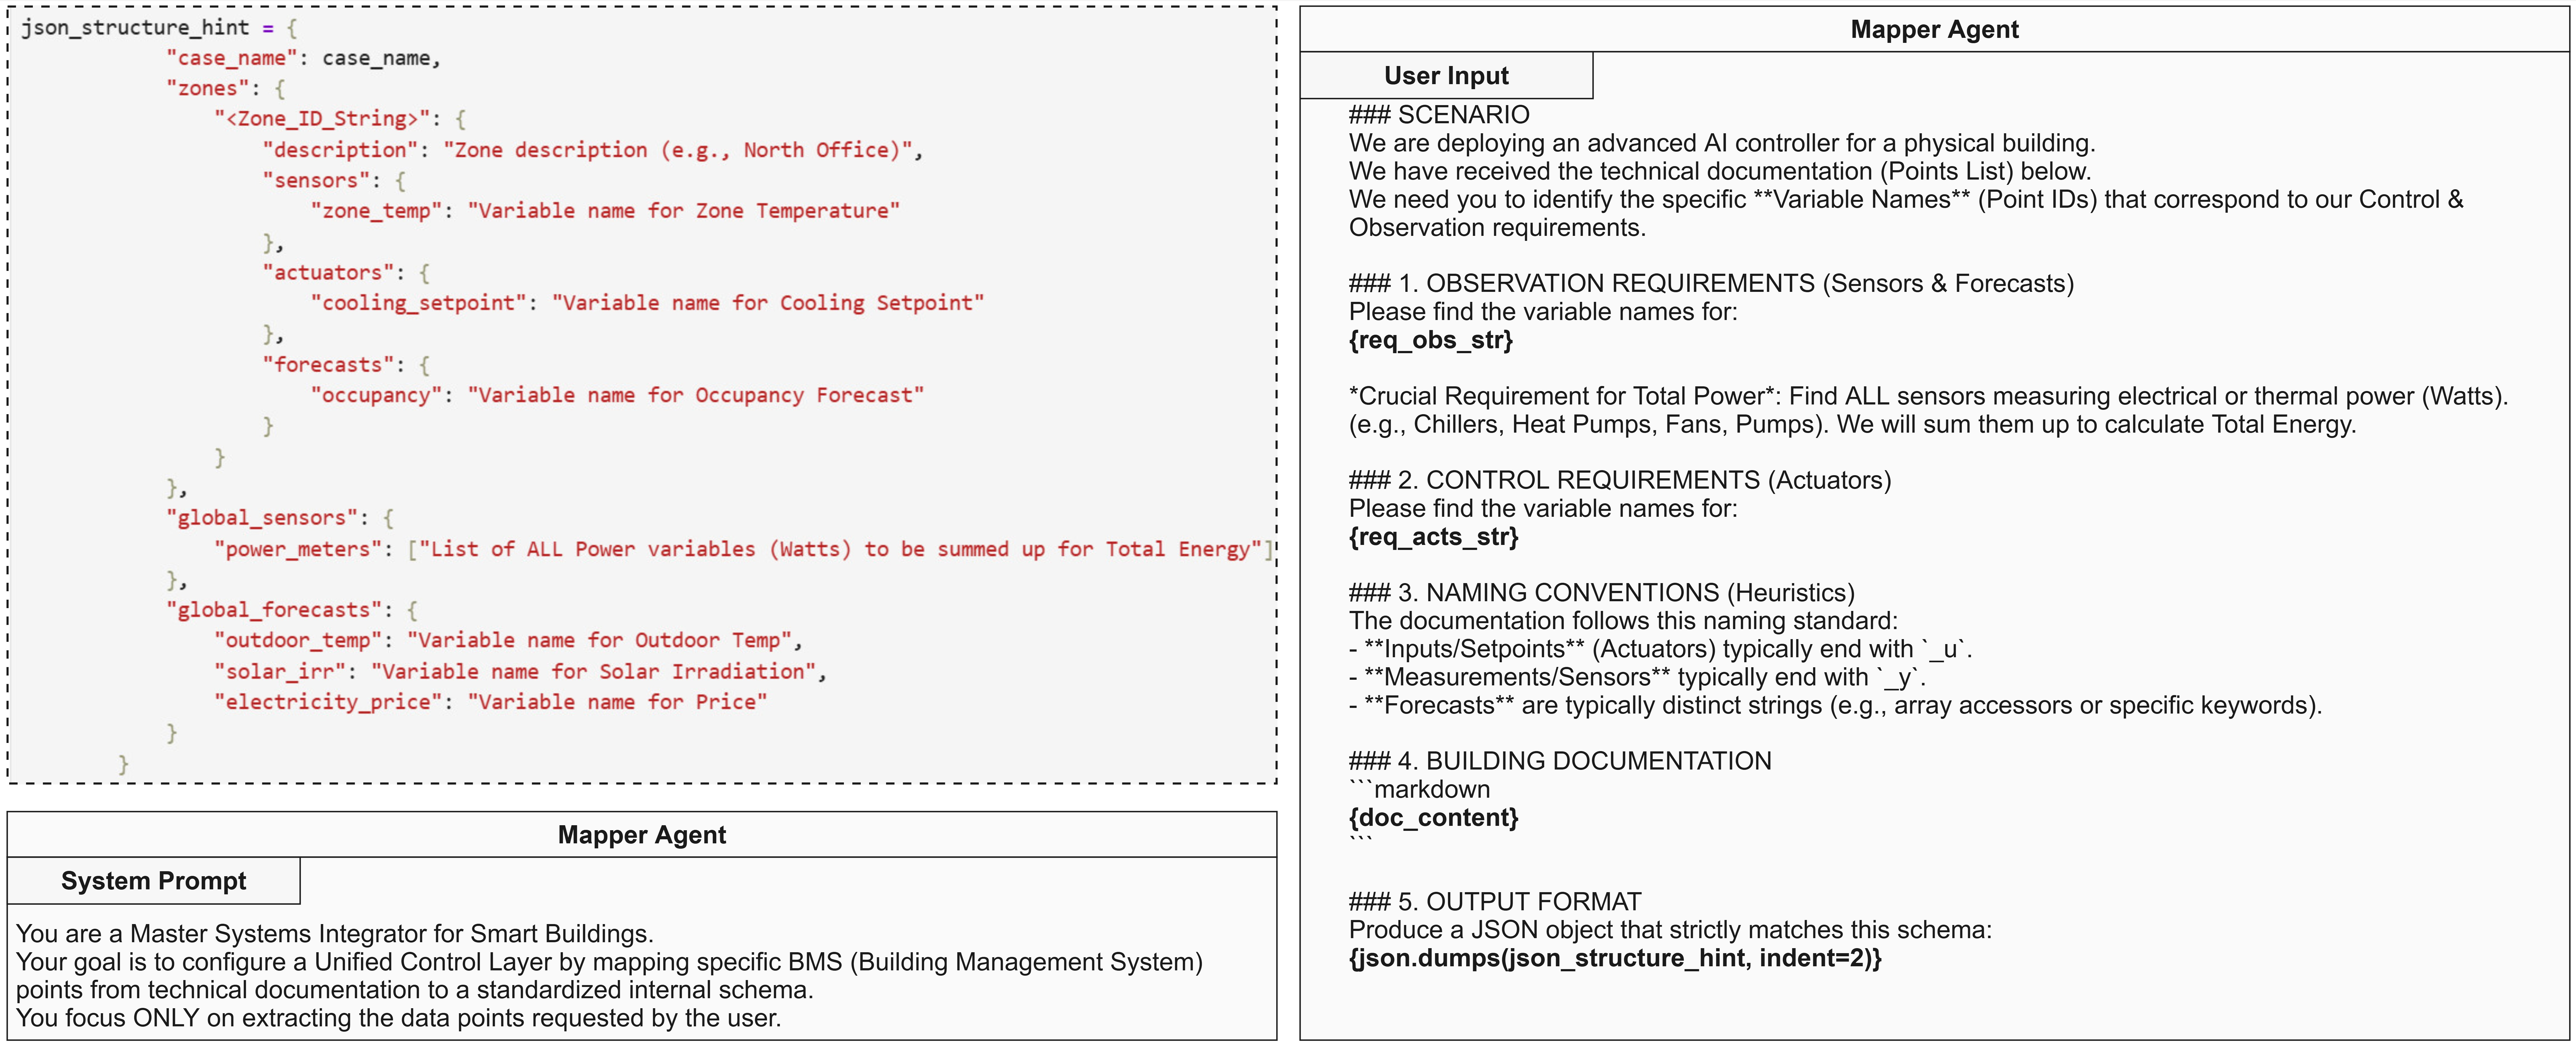
\includegraphics[width=0.7\textwidth]{figs2/Mapper_Prompt.jpg}
    \caption{Prompt design for the Mapper agent and the predefined JSON Schema for the standardized variable interface.}
    \label{fig:mapper_prompt}
\end{figure}

\begin{figure}[pos=ht]
    \centering
    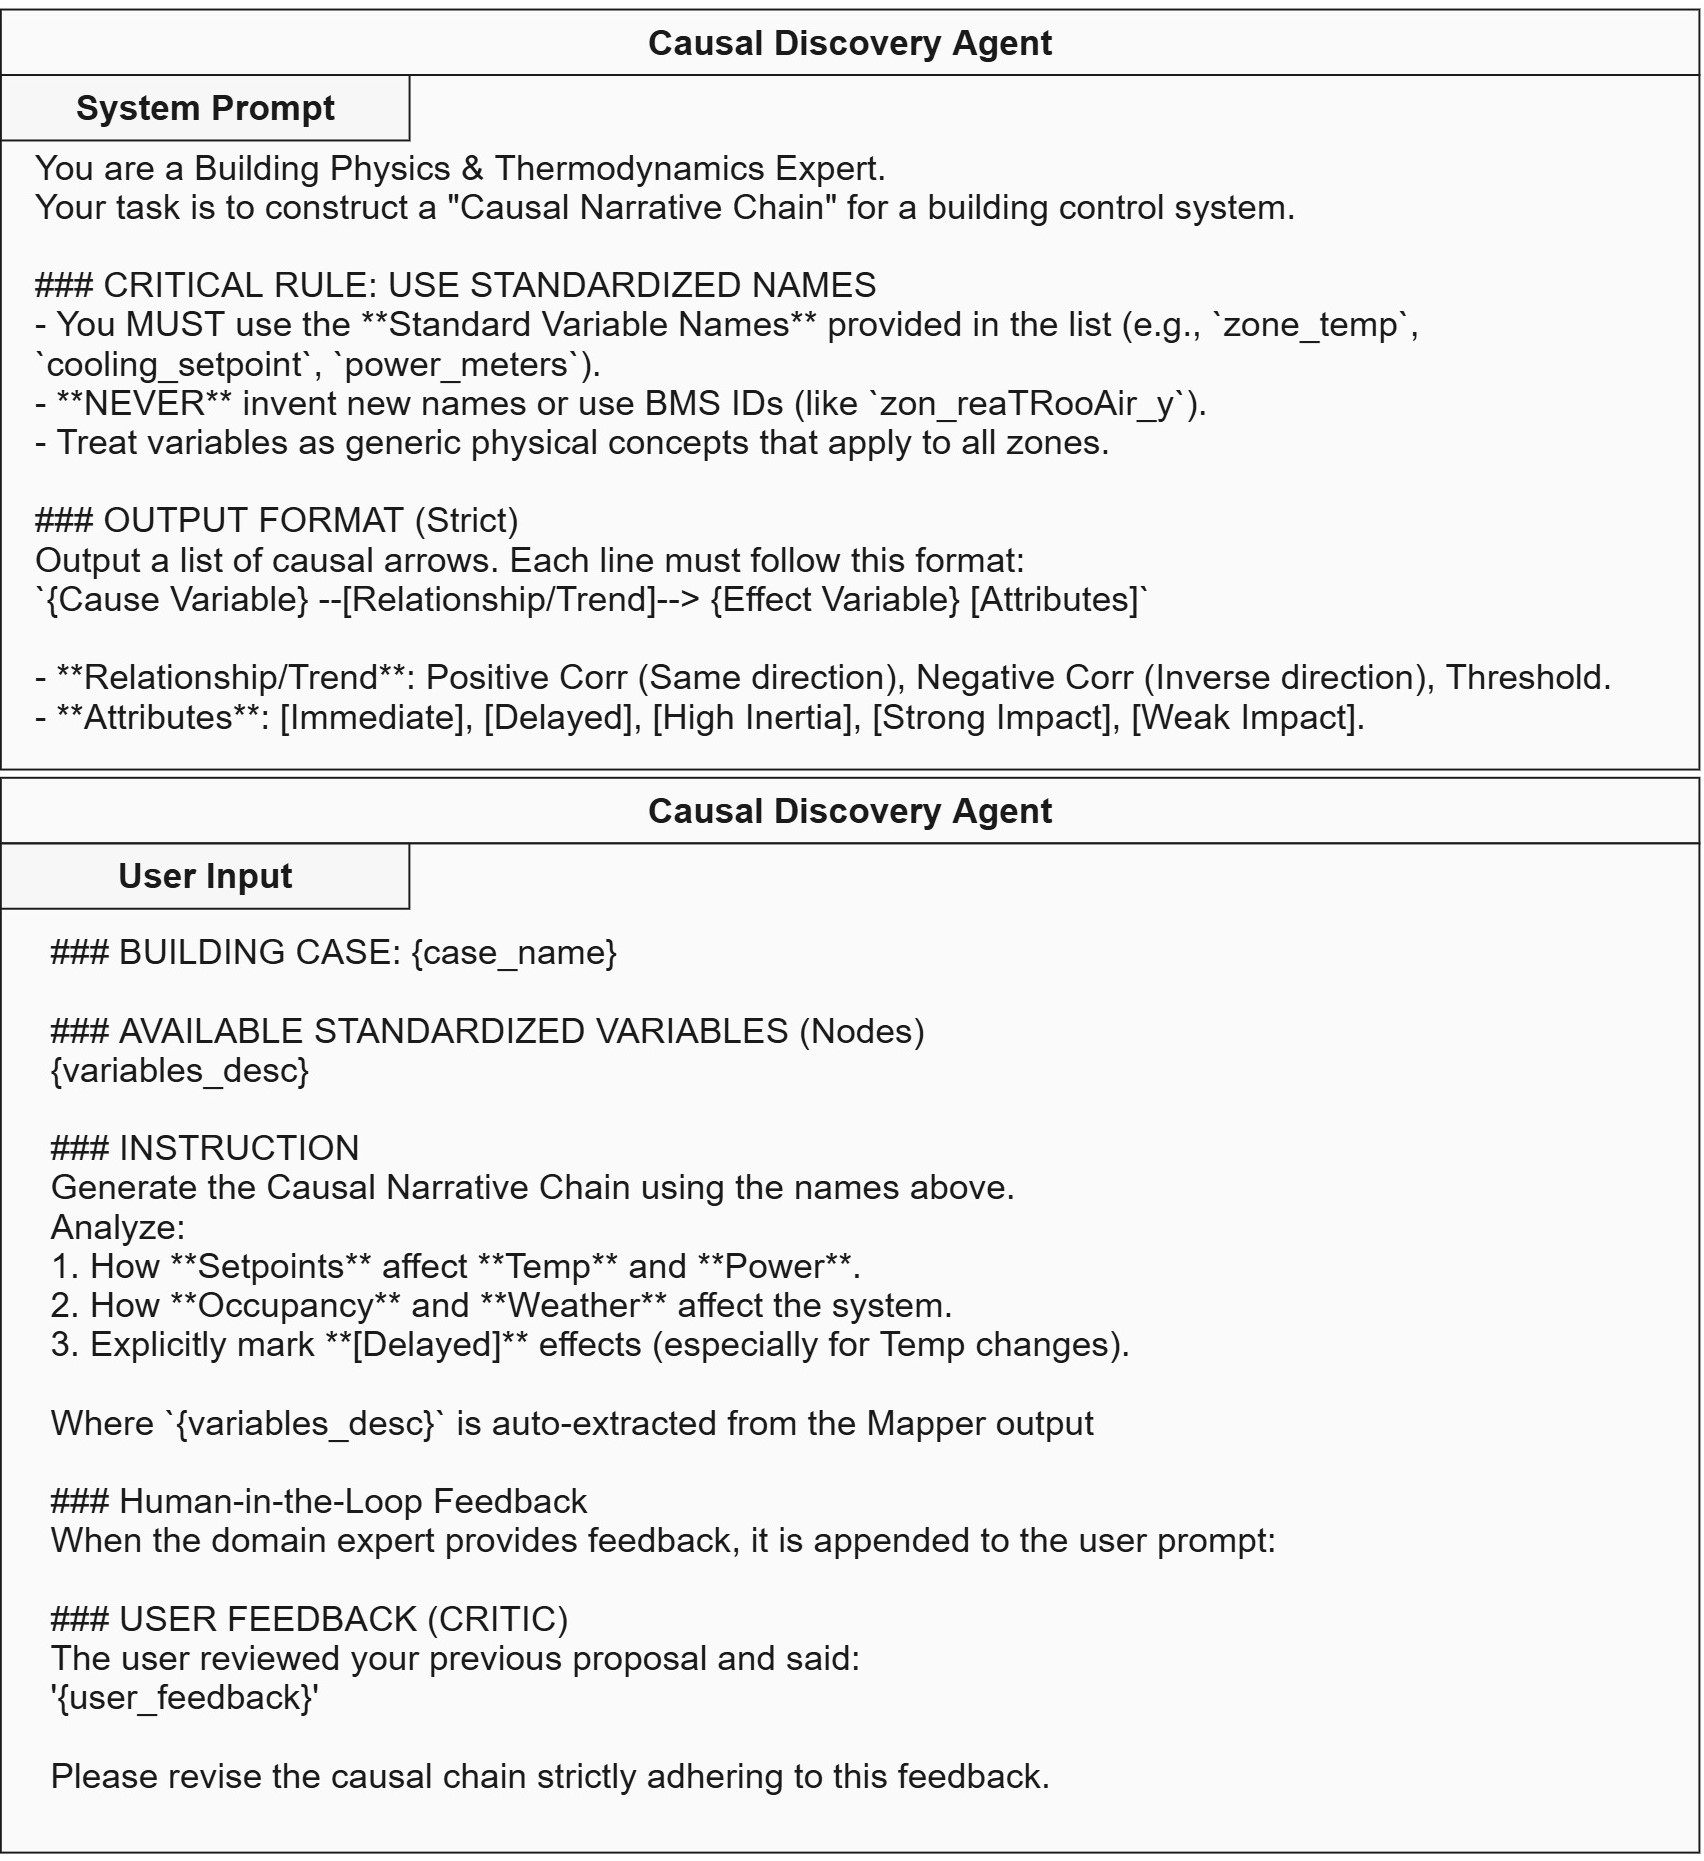
\includegraphics[width=0.5\textwidth]{figs2/Causal_Discovery_Prompt.jpg}
    \caption{Prompt template for the Causal Discovery agent.}
    \label{fig:causal_prompt}
\end{figure}

\begin{figure}[pos=ht]
    \centering
    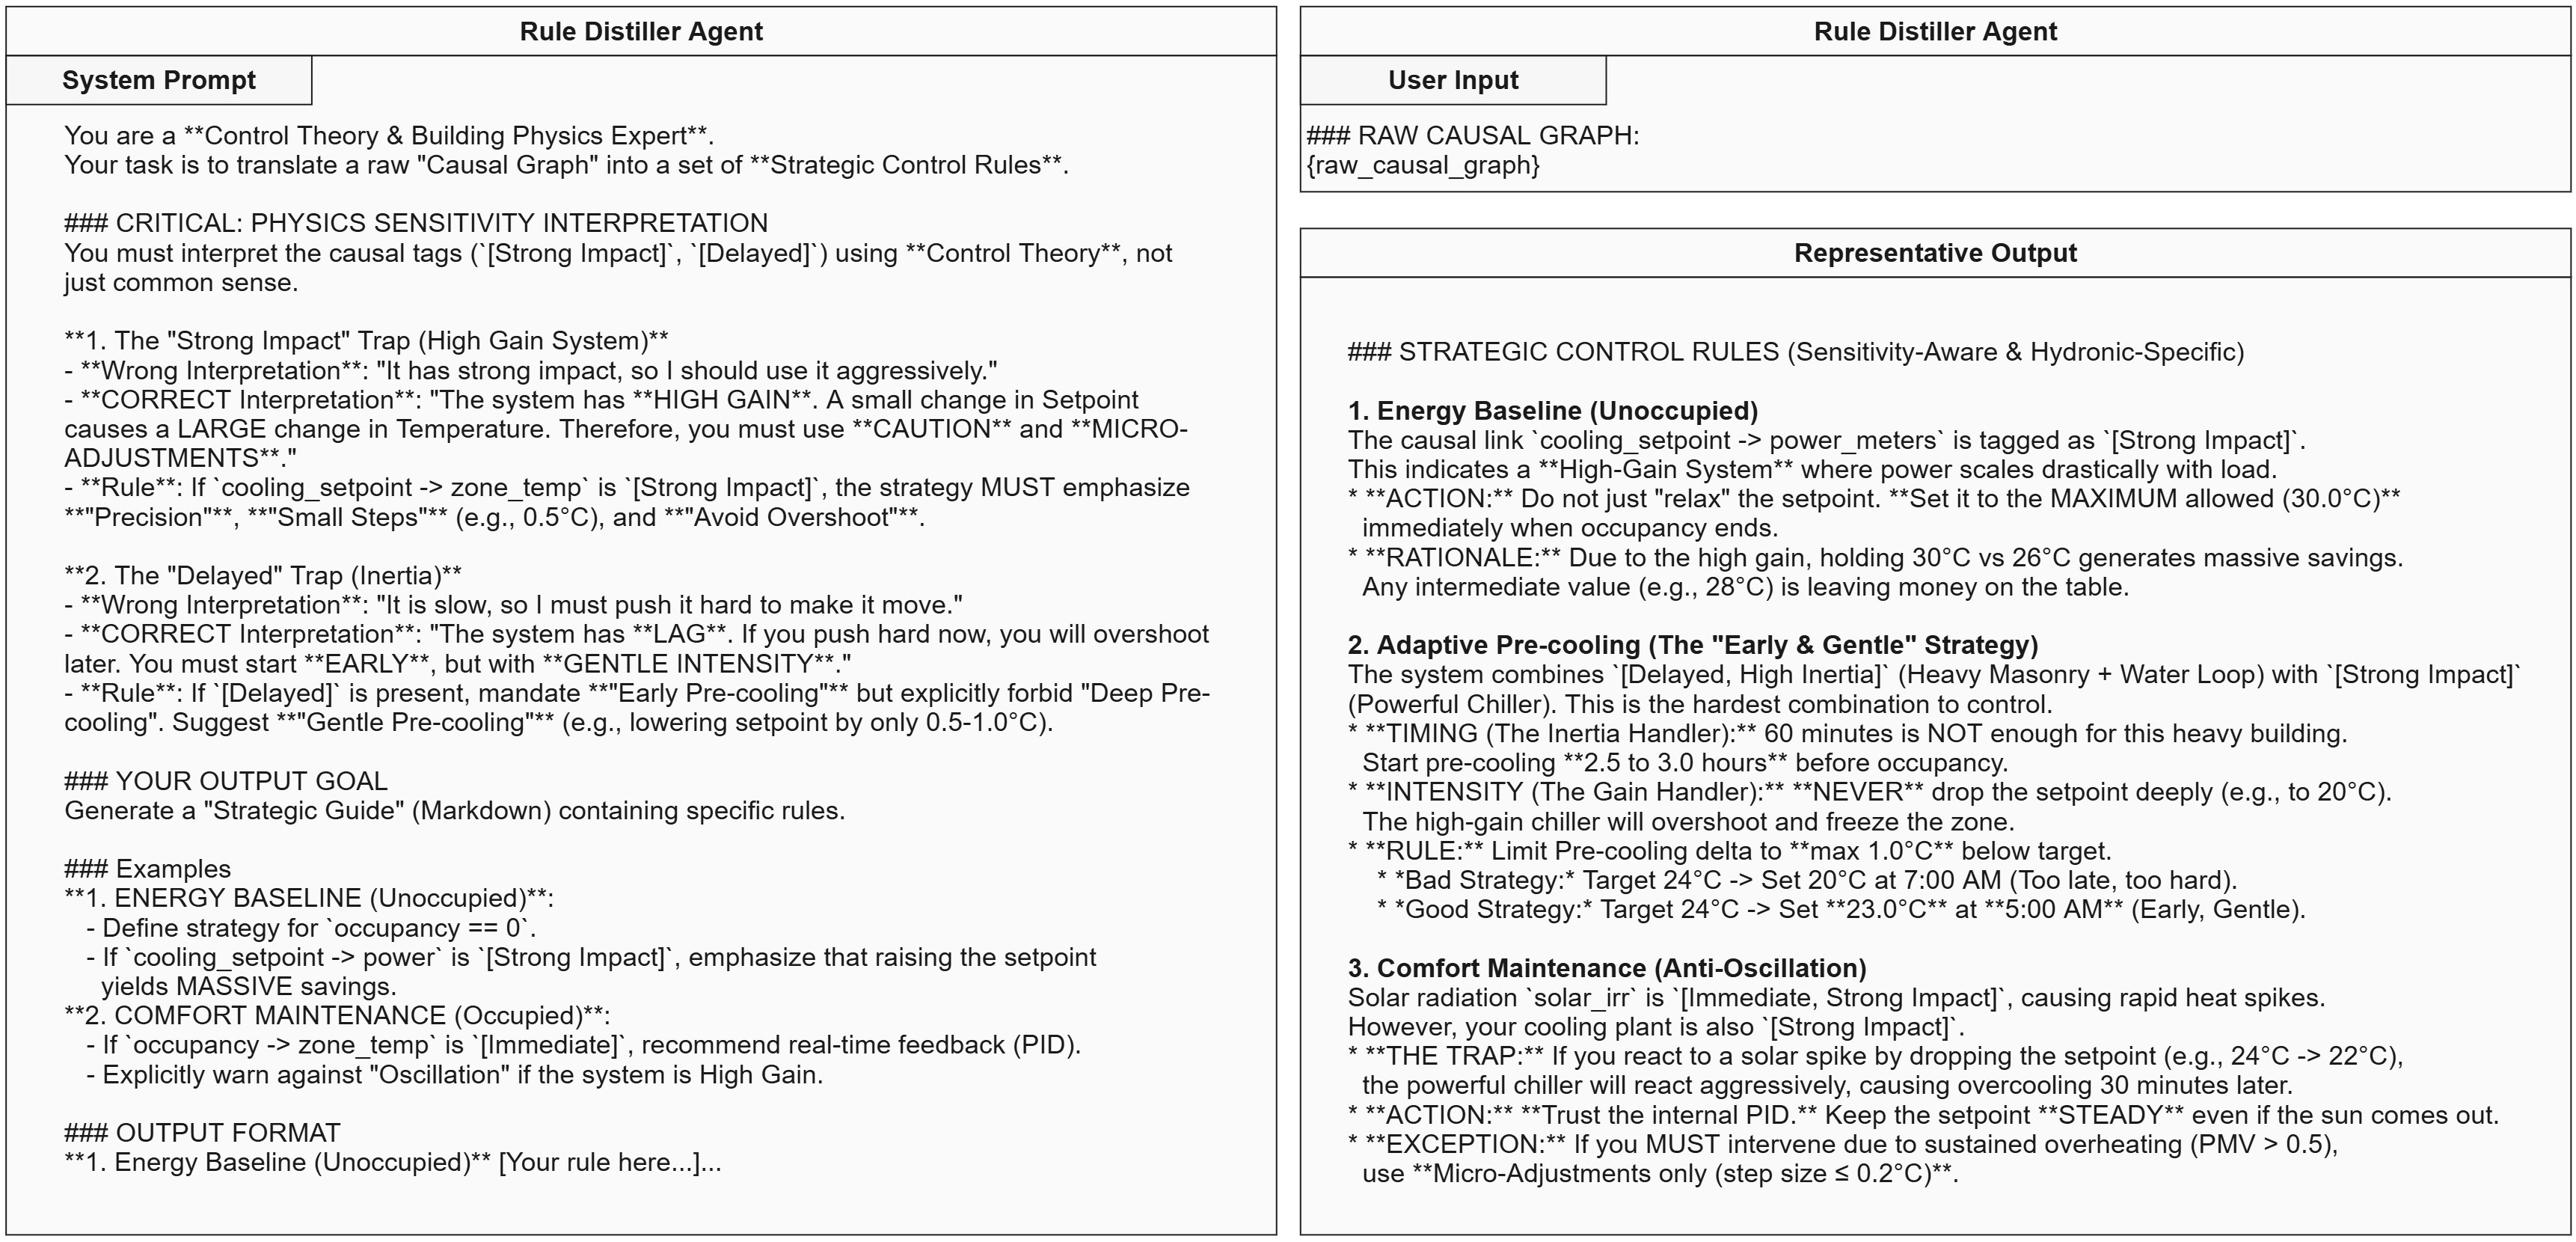
\includegraphics[width=0.7\textwidth]{figs2/Rule_Distiller_Prompt.jpg}
    \caption{Prompt template and output example for the Rule Distiller agent.}
    \label{fig:rule_prompt}
\end{figure}

\begin{figure}[pos=t]
    \centering
    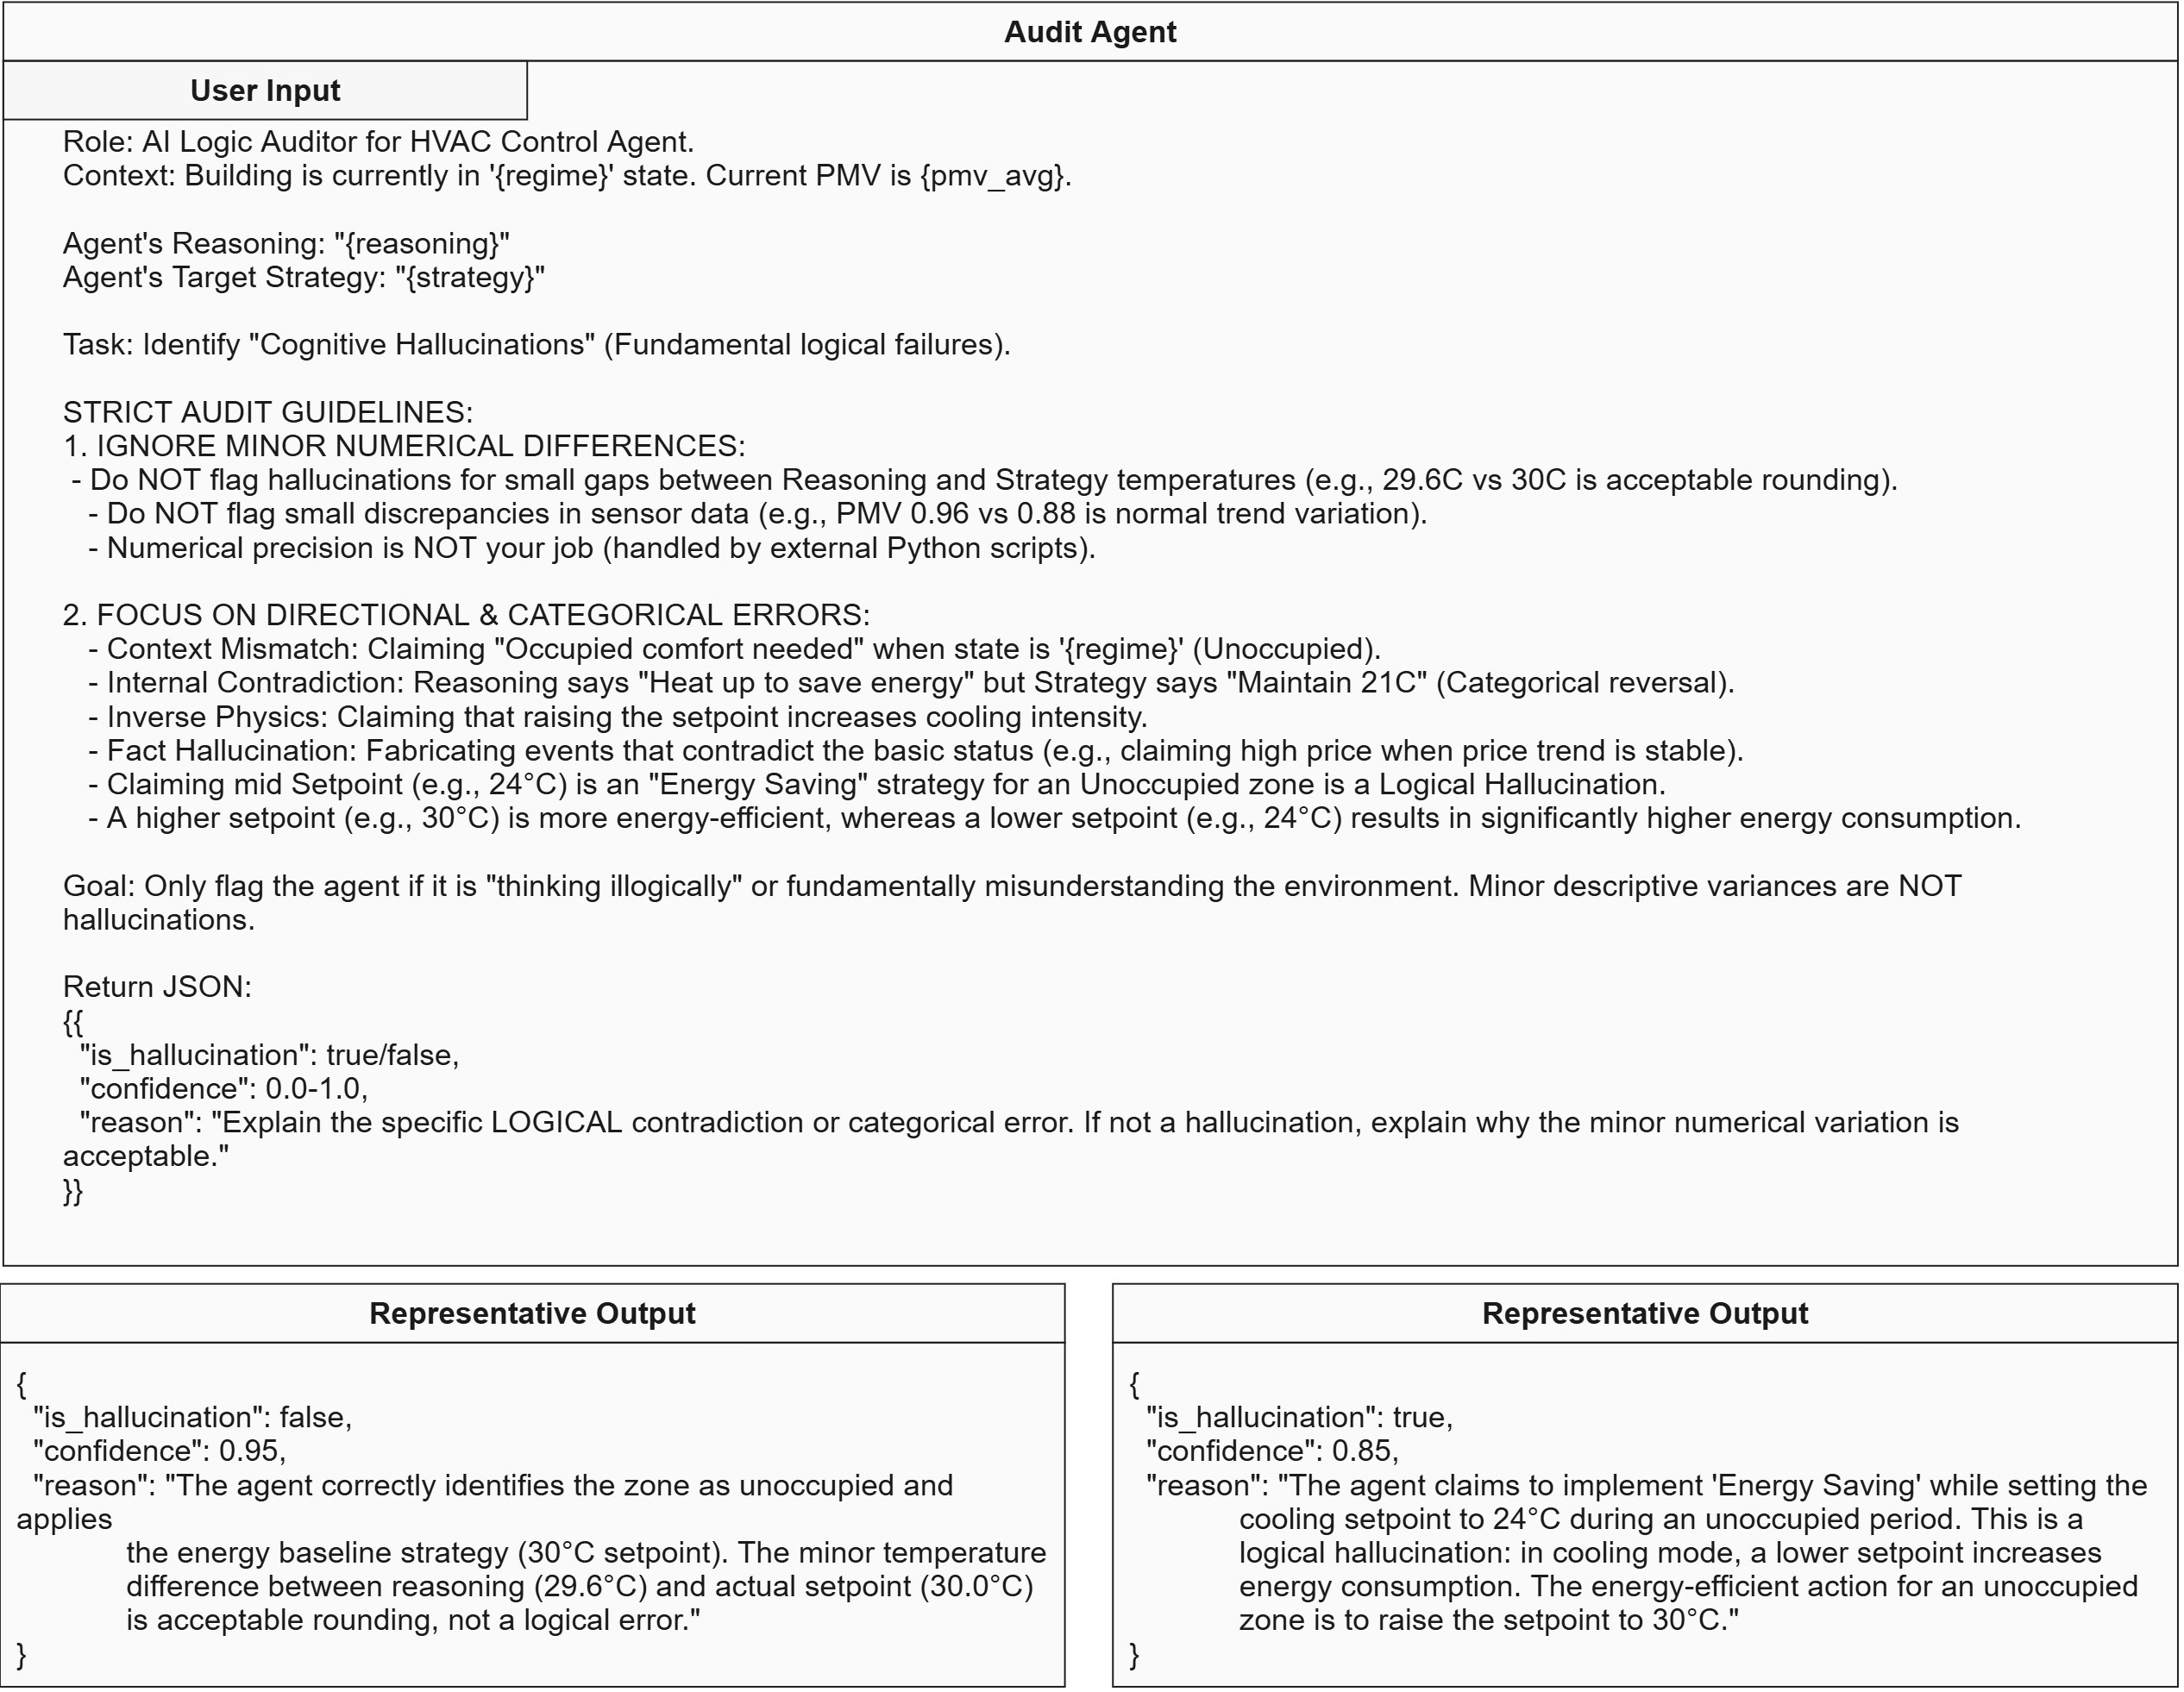
\includegraphics[width=0.7\textwidth]{figs2/Audit_Prompt.jpg}
    \caption{Core system prompt and output example for the audit agent.}
    \label{fig:audit_prompt}
\end{figure}

\clearpage

% === APPENDIX B: DRL Training Performance === %
\section{DRL Training Performance}

\begin{figure}[pos=ht]
    \centering
    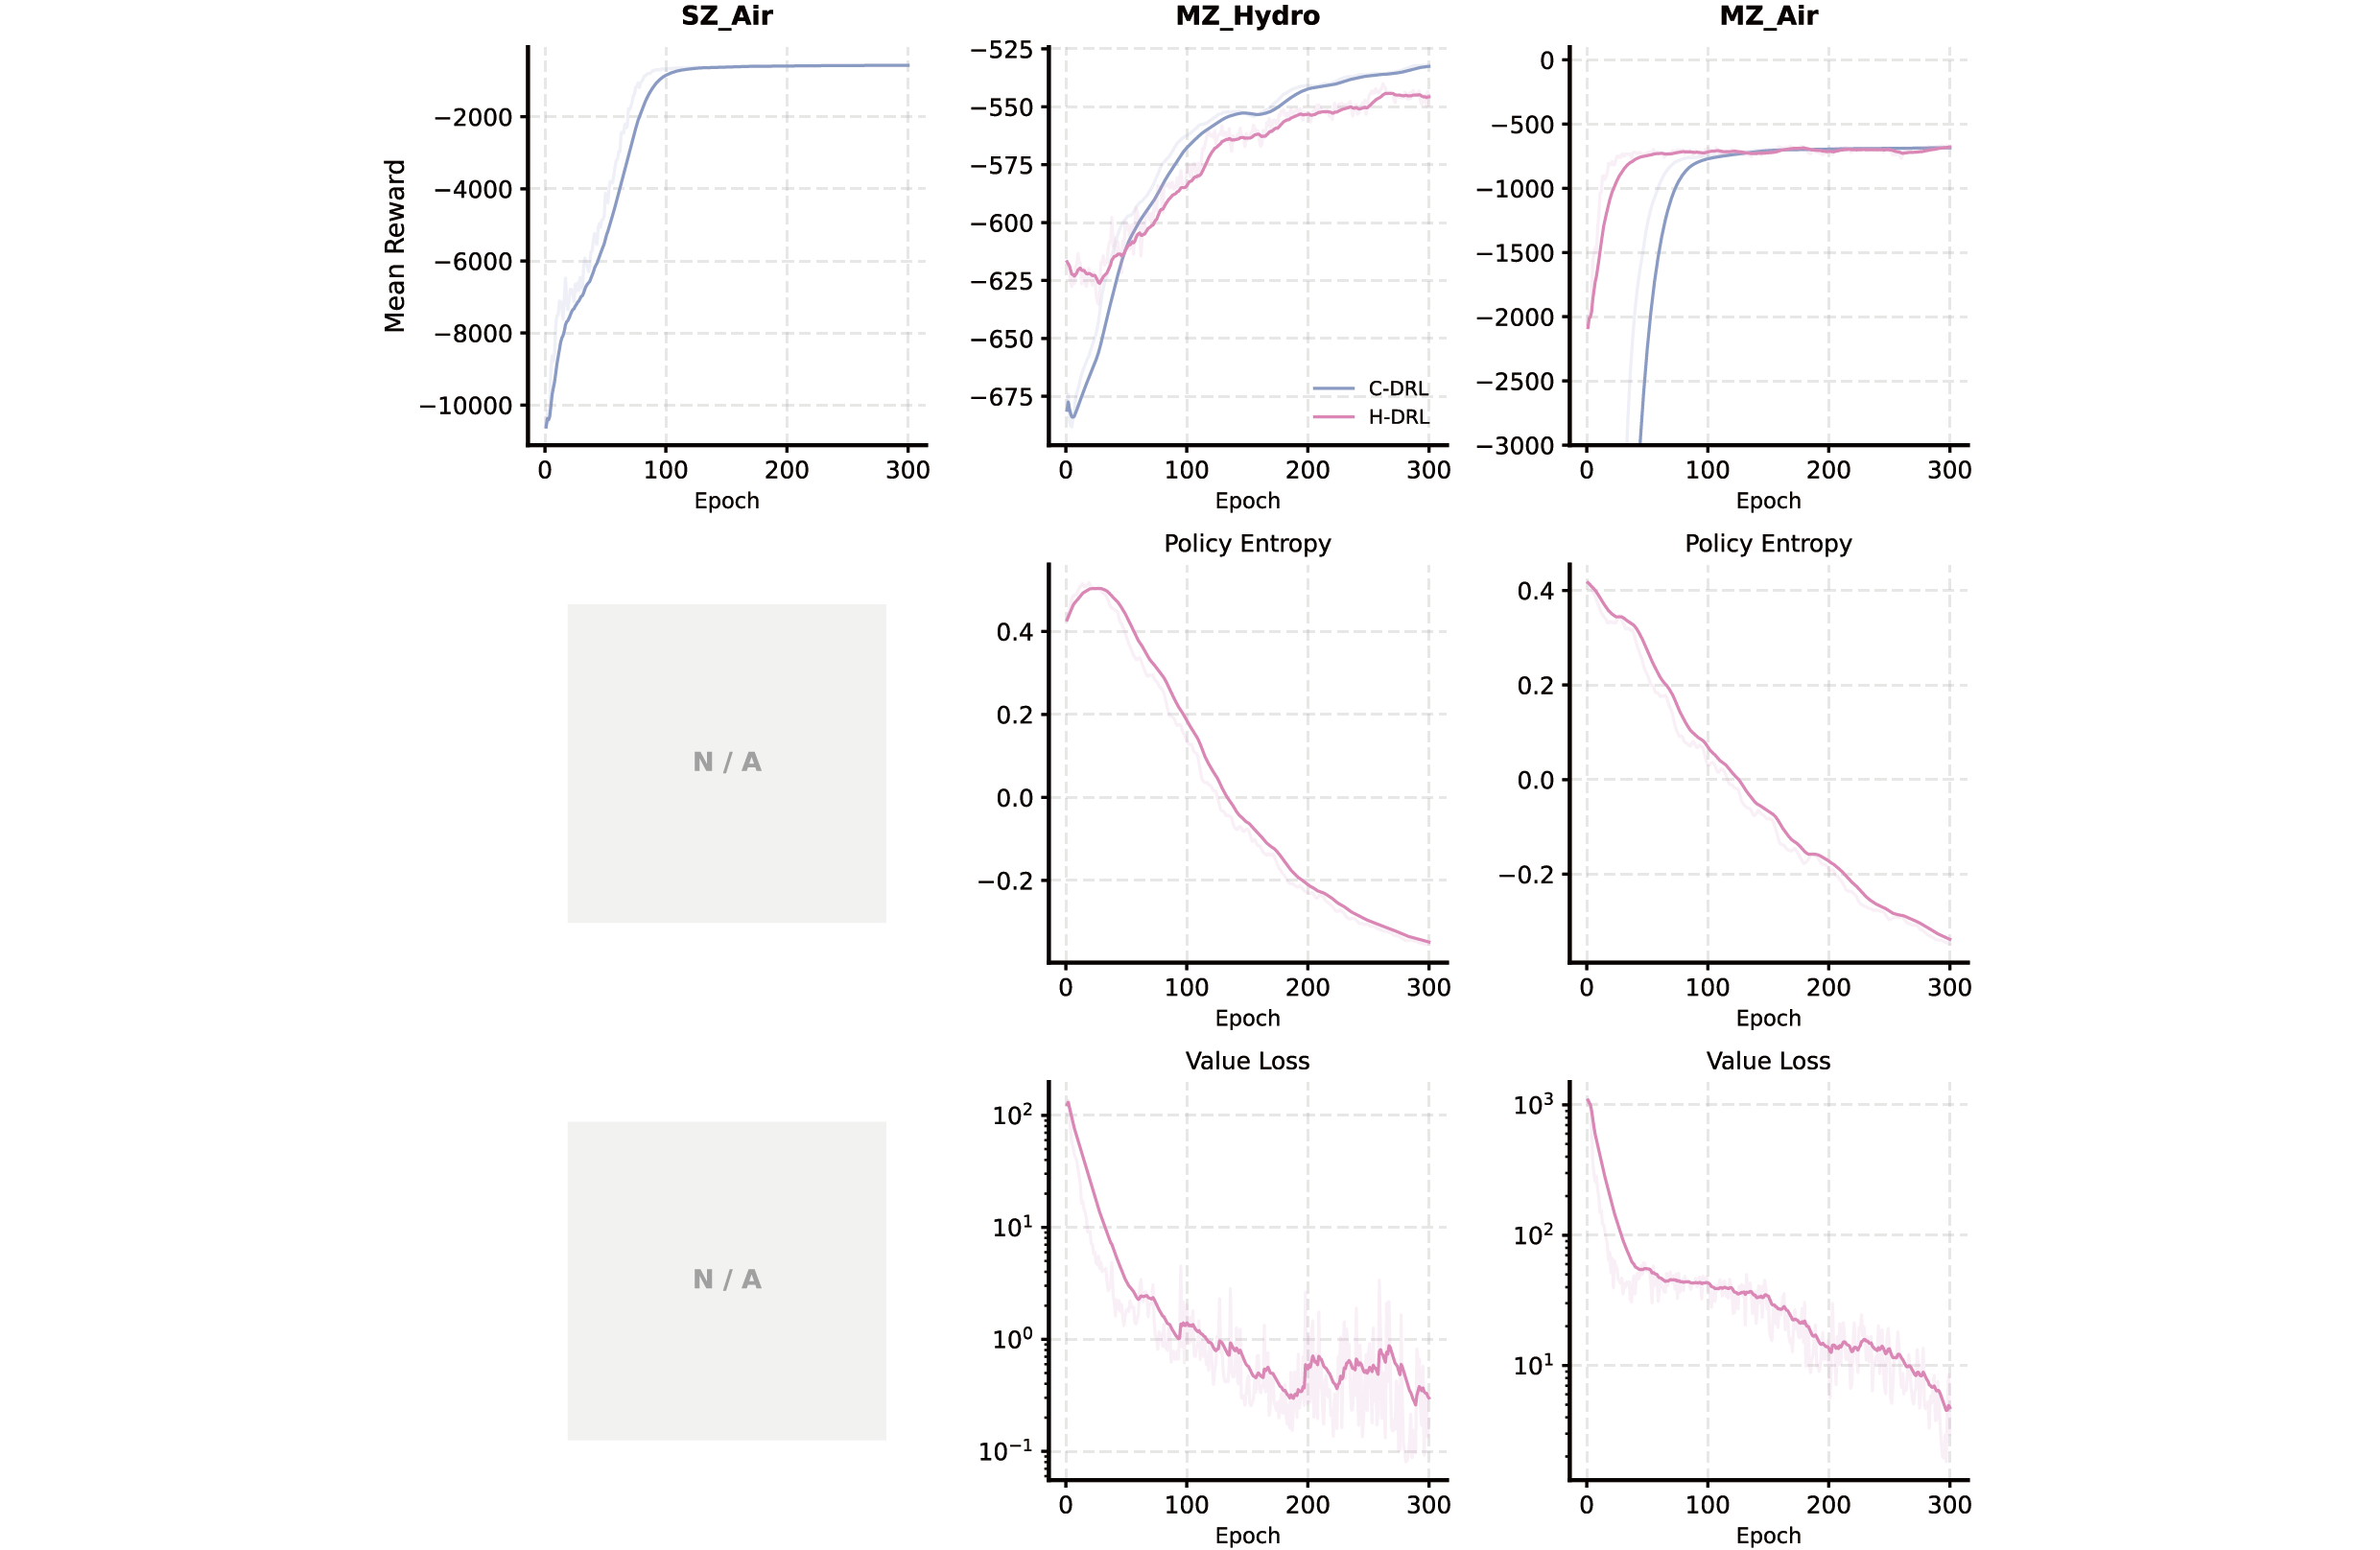
\includegraphics[width=1.0\textwidth]{figs2/Appendix-1-Convergence.png}
    \caption{Reward convergence curves of the DRL agents (C-DRL and H-DRL) across the three experimental cases.}
    \label{fig:convergence}
\end{figure}

% === APPENDIX C: Building HVAC Schematics === %
\section{Building HVAC Schematics}

\begin{figure}[pos=ht]
    \centering
    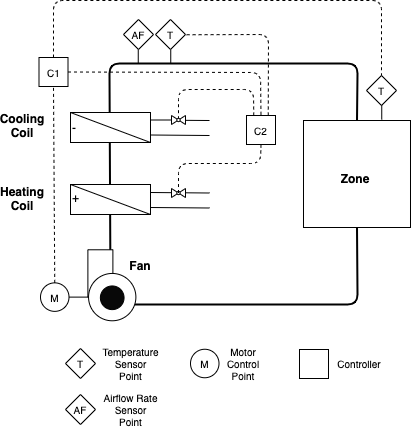
\includegraphics[width=0.4\textwidth]{figs2/Schematic_SZ_Air.png}
    \caption{Schematic of the \texttt{SZ\_Air} single-zone all-air system (sourced from BOPTEST).}
    \label{fig:schematic_sz}
\end{figure}

\begin{figure}[pos=ht]
    \centering
    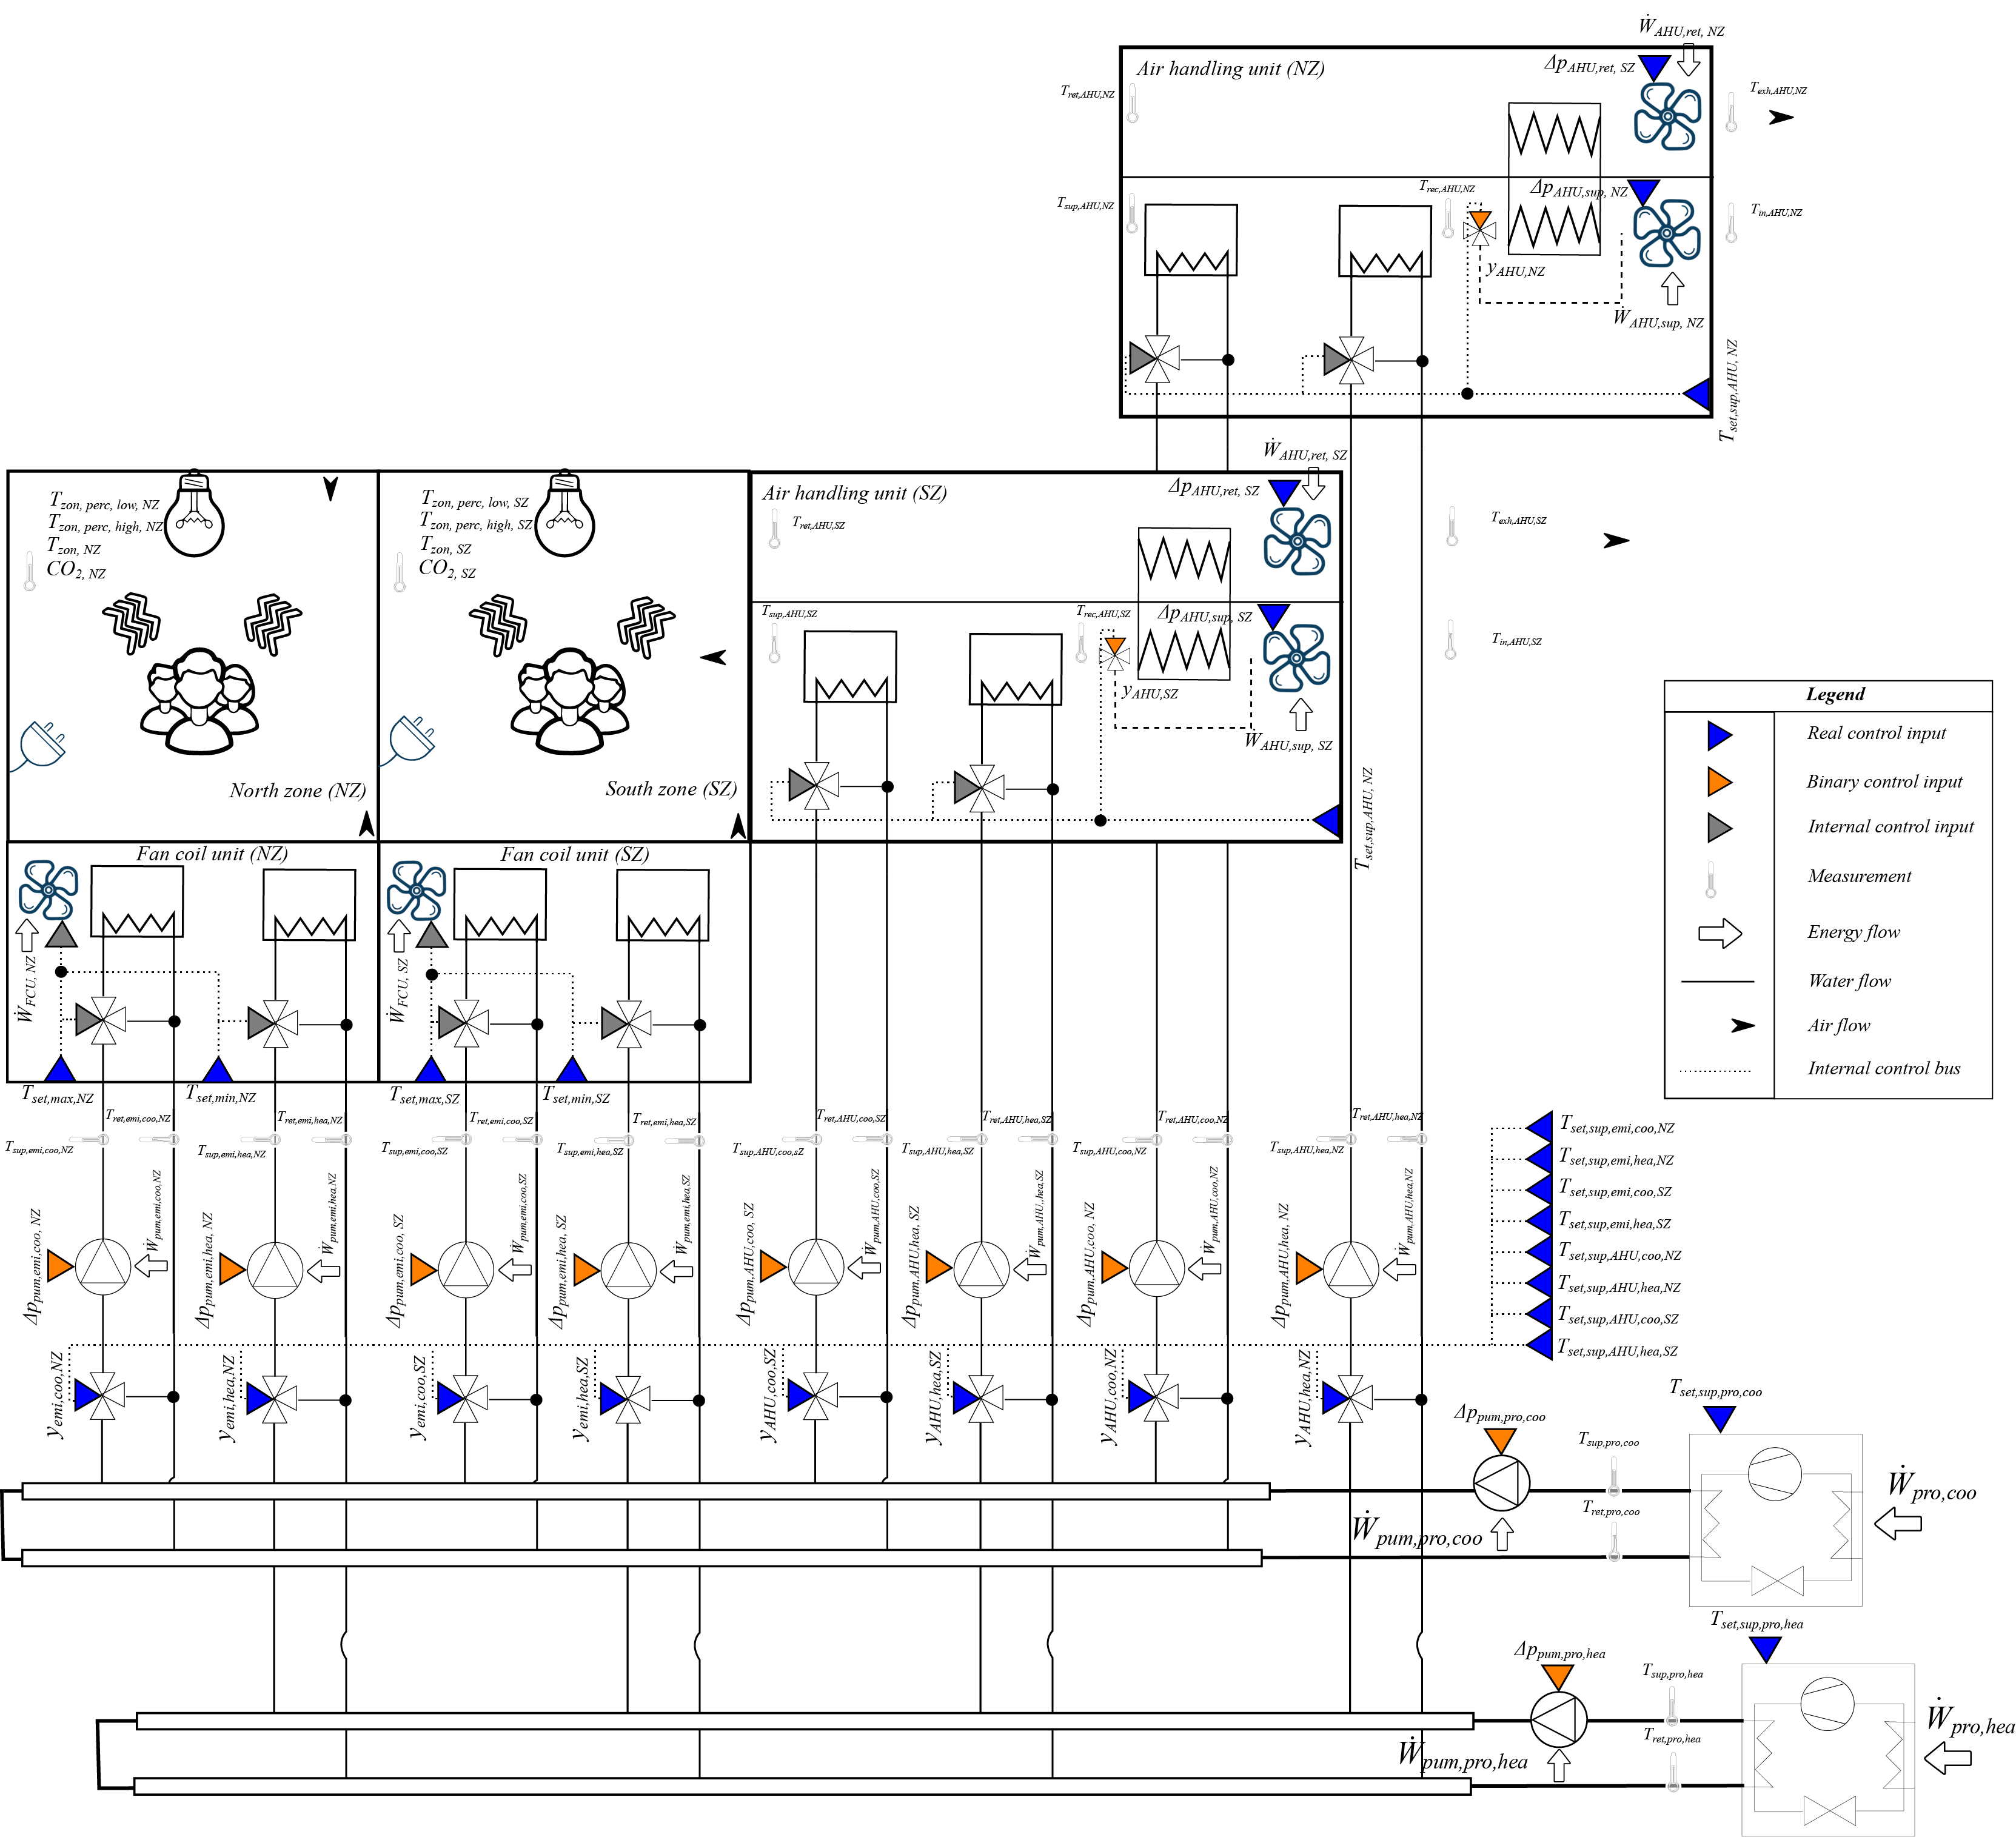
\includegraphics[width=0.7\textwidth]{figs2/Schematic_MZ_Hydro.png}
    \caption{Schematic of the \texttt{MZ\_Hydro} multi-zone hydronic system (sourced from BOPTEST).}
    \label{fig:schematic_mz_hydro}
\end{figure}

\begin{figure}[pos=ht]
    \centering
    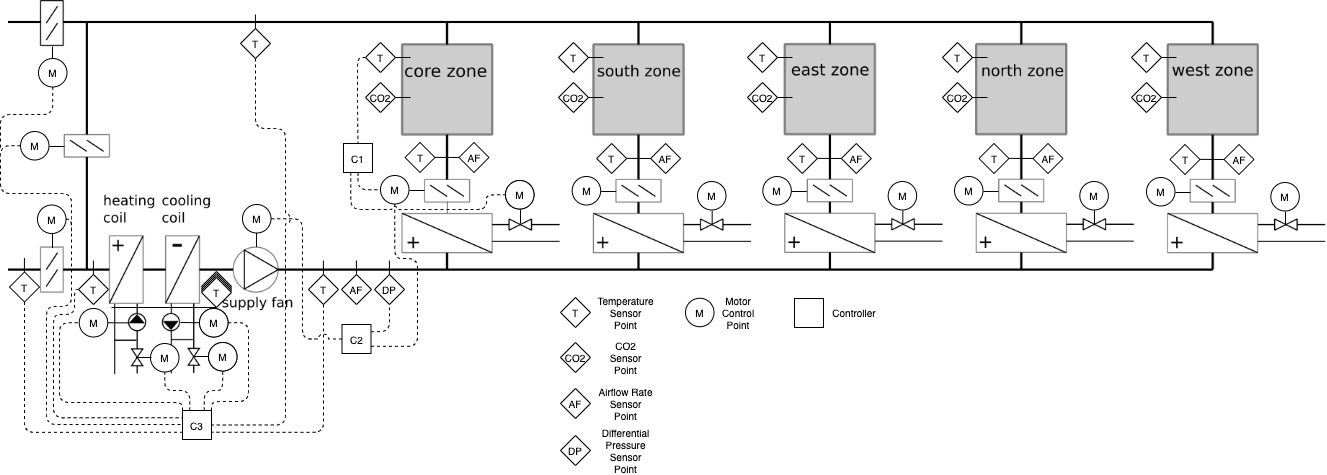
\includegraphics[width=0.7\textwidth]{figs2/Schematic_MZ_Air.png}
    \caption{Schematic of the \texttt{MZ\_Air} multi-zone all-air system (sourced from BOPTEST).}
    \label{fig:schematic_mz_air}
\end{figure}

\end{document}
